\documentclass[10pt, a4paper]{article}
\usepackage[utf8]{inputenc}
\usepackage[paper=a4paper, left=1.5cm, right=1.5cm, bottom=1.5cm, top=3.5cm]{geometry}
\usepackage[spanish]{babel}
\usepackage{indentfirst}
\usepackage{fancyhdr}
\usepackage{latexsym}
\usepackage{lastpage}
\usepackage[colorlinks=true, linkcolor=blue]{hyperref}
\usepackage{calc}
\usepackage{verbatim}
\usepackage{listings}
\usepackage{amsfonts}
\usepackage{float}
\setcounter{tocdepth}{5}
\usepackage{caption}
\usepackage{subcaption}
\sloppy

\parskip=5pt % 10pt es el tamaño de fuente

% Pongo en 0 la distancia extra entre ítemes.
\let\olditemize\itemize
\def\itemize{\olditemize\itemsep=0pt}

\usepackage{caratula}

% Acomodo fancyhdr.
\pagestyle{fancy}
\thispagestyle{fancy}
\addtolength{\headheight}{1pt}
\lhead{S. Aboy Solanes, E. Almansi, F. Canay, F. Decroix}
\rhead{$2^{\mathrm{do}}$ cuatrimestre de 2014}
\cfoot{\thepage /\pageref{LastPage}}
\rfoot{Trabajo Práctico 1 - Wiretapping}
\renewcommand{\footrulewidth}{0.4pt}

\begin{document}


\titulo{Trabajo Práctico 1 - Wiretapping}
\fecha{Martes 23 de Septiembre}
\materia{Teoría de las Comunicaciones}
\integrante{Santiago Aboy Solanes}{175/12}{santiaboy2@hotmail.com}
\integrante{Emilio Almansi}{674/12}{ealmansi@gmail.com}
\integrante{Federico Canay}{250/12}{fcanay@hotmail.com}
\integrante{Facundo Decroix}{842/11}{fndecroix92@hotmail.com}

%Pagina de titulo e indice
\thispagestyle{empty}

\maketitle

%\thispagestyle{empty}
%\mbox{}
%\newpage
\thispagestyle{empty}
\tableofcontents

\newpage

\section{Introducción}
\label{sec:introduccion}
En este trabajo práctico vamos a abordar el desarrollo de herramientas de diagnóstico de red. Nuestro objetivo va a ser analizar estadísticamente el protocolo ARP. Por otro lado, vamos a sacar conclusiones acerca de los tipos de dispositivos de red que se pueden encontrar en un segumento de red determinado. Para ello, utilizamos la herramienta de manipulación y análisis de paquetes, Scapy.

\section{Desarrollo}
\label{sec:desarrollo}
Antes de comenzar el desarrollo vamos a definir algunos términos.

$\bullet$ \textbf{Nodo distinguido}: En una fuente, un nodo distinguido es un nodo cuya información es menor a la entropía de dicha fuente.

\subsection{Capturando tráfico}
Para el desarrollo de este trabajo práctico escuchamos pasivamente redes para poder observar que sucedía en las mismas. En particular, capturamos paquetes ARP \emph{who-has}.

Utilizamos dos modelos de fuente de información:

$S_{dst}$ = \{$s_1$ $\cdots$ $s_n$\} siendo $s_i$ una IP que aparece como dirección destino en los paquetes ARP \emph{who-has}

$S_{src}$ = \{$s_1$ $\cdots$ $s_n$\} siendo $s_i$ una IP que aparece como dirección origen en los paquetes ARP \emph{who-has}

Creamos una \emph{tool} que escucha pasivamente en la red local. Luego, la adaptamos para que estime las probabilidades de dichas fuentes en función de los paquetes ARP observados y que calcule la entropía de las mismas.

Usando dicha herramienta, realizamos capturas de paquetes ARP sobre distintas LANs: Alto Palermo, Red laboral de Honeywell, Laboratorios de Ciudad Universitaria (Via Wi-Fi), y la casa de un integrante del grupo.

\subsection{Gráficos}

Una vez que capturamos el tráfico, nos propusimos gráficar y a analizar los datos obtenidos. Realizamos tres tipos de gráficos:

$\bullet$ Grafos dirigidos:
  En los grafos, los nodos son los IPs que aparecen en alguno de los paquetes capturados.
  Una arista entre A y B significa que se encontro un paquete con \emph{src} A y \emph{dst} B. El peso de cada arista corresponde a la cantidad de paquetes de la forma anterior.
  
  Ejemplo:
  
  \begin{figure}[H]
  \begin{center}
    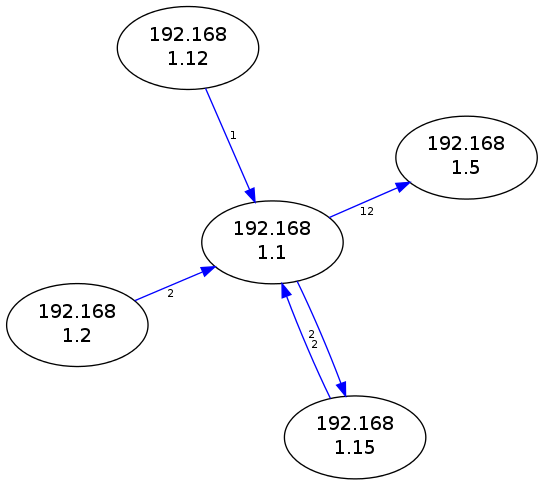
\includegraphics[width=0.3\linewidth]{../imgs/red-hogarena_red.png}
    \label{fig:FedeGrafo}
    \caption{Grafo de LAN hogareña}
  \end{center}
\end{figure}

$\bullet$ Histograma:
  Realizamos para cada una de las fuentes (\emph{src} y \emph{dst}), realizamos un histograma que muestra la cantidad de apariciones de un determinado IP en la fuente.
  
  Ejemplo:
  
  \begin{figure}[H]
  \begin{center}
    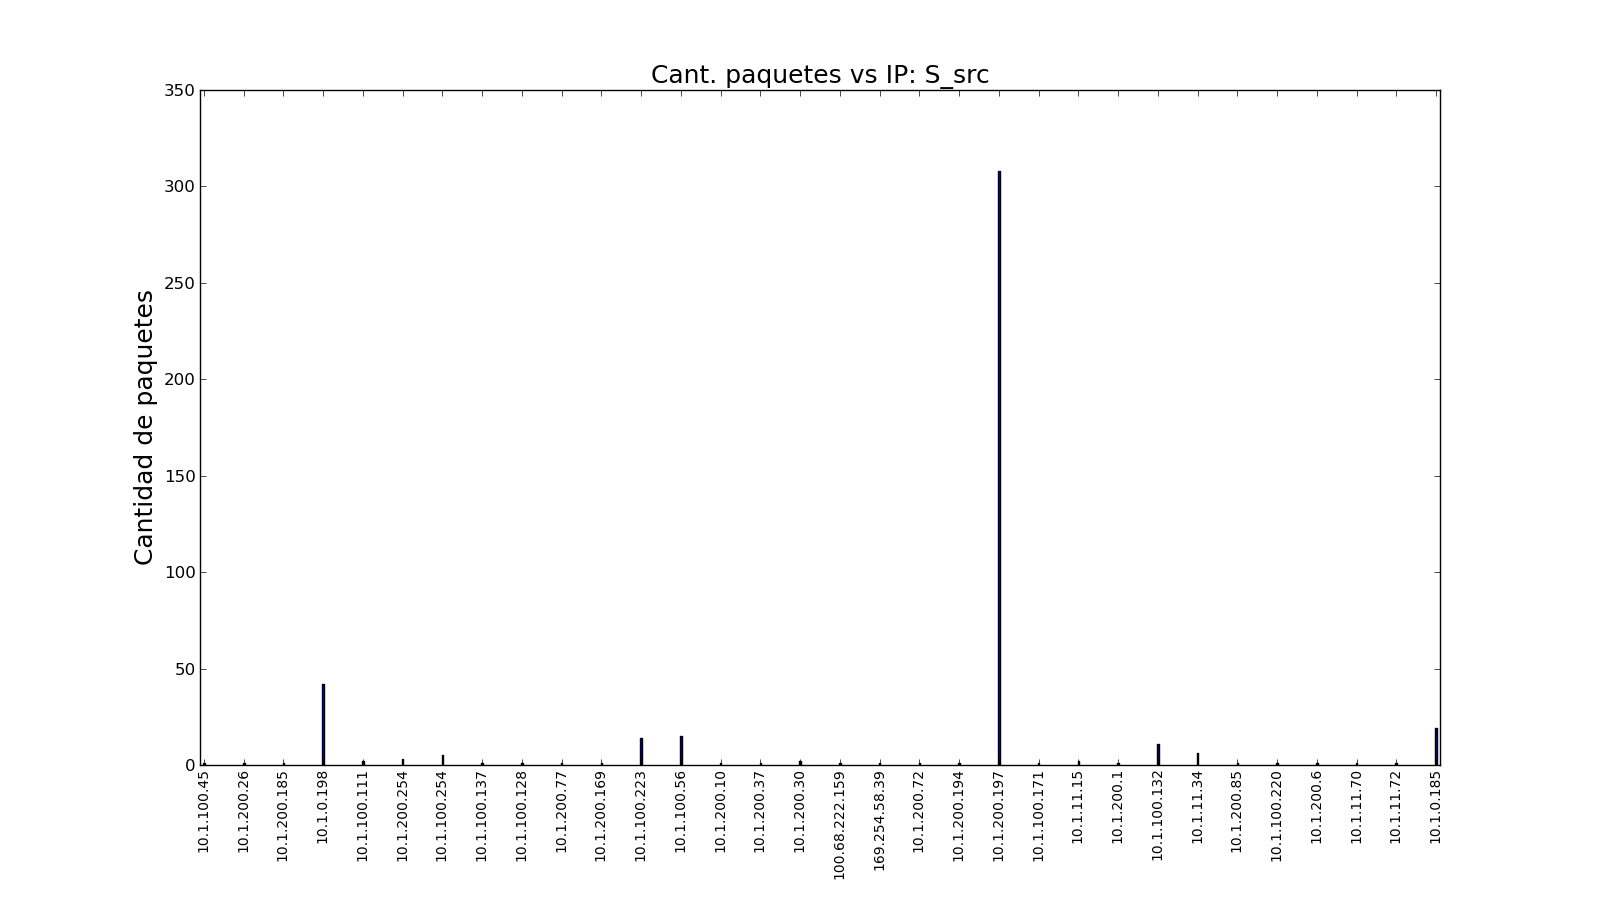
\includegraphics[width=0.8\linewidth]{../imgs/red-entrepiso-dc_S_src_hist.png}
    \caption{Histograma de la serie de paquetes s\_src de la red \emph{Entrepiso-DC}.}
    \label{fig:histograma-entrepiso-dc-s-src}
  \end{center}
  \end{figure}
  
$\bullet$ Gráfico Información:
  Realizamos para cada una de las fuentes (\emph{src} y \emph{dst}), realizamos un gráfico donde se muestra la información de un determinado IP en la fuente. Además graficamos una recta con el valor de la entropía para comparar facilmente la información de cada IP con la entropía de la fuente. 
  
  Ejemplo:
  
  \begin{figure}  
  \begin{center}
    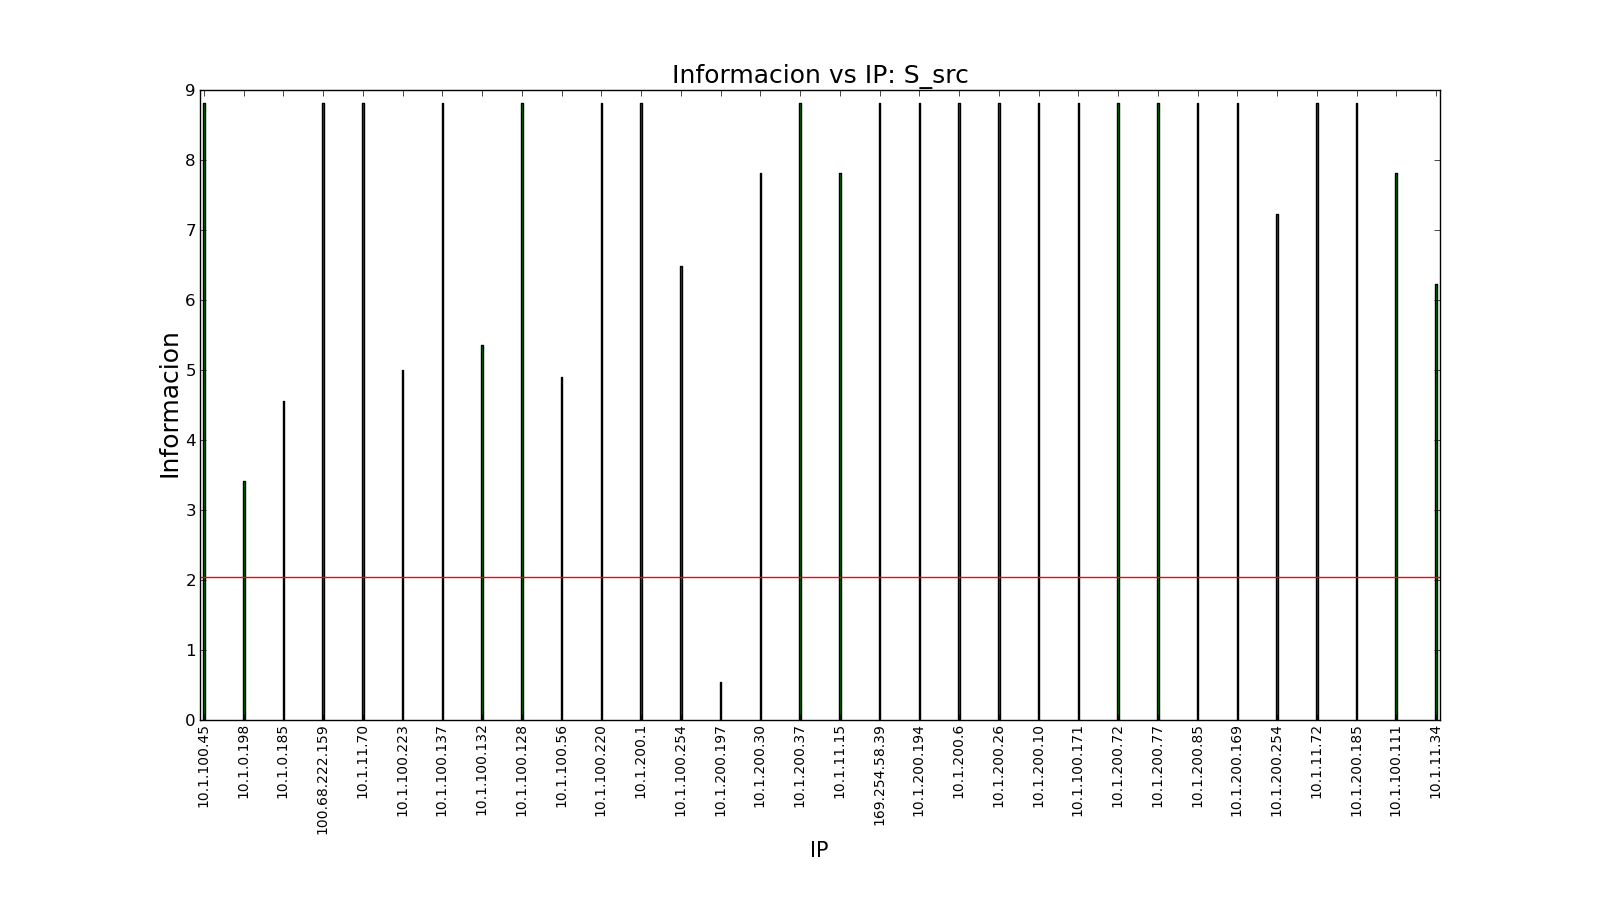
\includegraphics[width=0.8\linewidth]{../imgs/red-entrepiso-dc_S_src_info.png}
    \caption{Gráfico de cantidad de información para cada IP s\_src de la red \emph{Entrepiso-DC}.}
    \label{fig:informacion-entrepiso-dc-s-src}
  \end{center}
\end{figure}
  
Graficamos en forma de histogramas, y de grafos la información y entropía de $S_{dst}$ y $S_{src}$

\section{Experimentación}
En cada una de las LANs mencionadas en la sección \ref{sec:introduccion}, utilizamos las herramientas desarrolladas para capturar el tráfico ARP, y posteriormente gráficar y analizar los datos obtenidos. Con la finalidad de reconocer los nodos distinguidos de cada red, realizamos los siguientes tres tipos de gráficos.

\subsection{Grafos dirigidos}

  Para representar gráficamente el grafo de relación entre los nodos de una muestra (sección \ref{subsec:grafo-relacion-nodos}), graficamos grafos dirigidos donde hay un nodo por cada IP que aparece en alguno de los paquetes capturados.
 
  Una arista entre los nodos A y B significa que se encontro un paquete con \emph{src} A y \emph{dst} B. El peso de cada arista corresponde a la cantidad de paquetes de la forma anterior.
  
  Por ejemplo, en la figura \ref{fig:FedeGrafo-ejemplo}, se observó un paquete con fuente \emph{192.168.1.12} y destino \emph{192.168.1.1}, y un total de 12 paquetes con fuente \emph{192.168.1.1} y destino \emph{192.168.1.5}.
  
  \begin{figure}[H]
  \begin{center}
    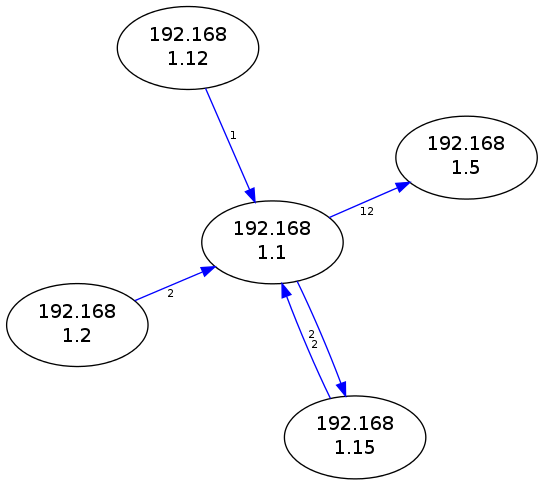
\includegraphics[width=0.3\linewidth]{../imgs/red-hogarena_red.png}
    \caption{Grafo de LAN hogareña}
    \label{fig:FedeGrafo-ejemplo}
  \end{center}
\end{figure}

\subsection{Histograma}

  En cada red y para cada una de las fuentes ($S_{src}$, $S_{dst}$), realizamos un histograma que muestra la cantidad de apariciones de un determinado IP en la fuente. Se muestra un ejemplo en la figura \ref{fig:histograma-entrepiso-dc-s-src-ejemplo}.
  
  \begin{figure}[H]
  \begin{center}
    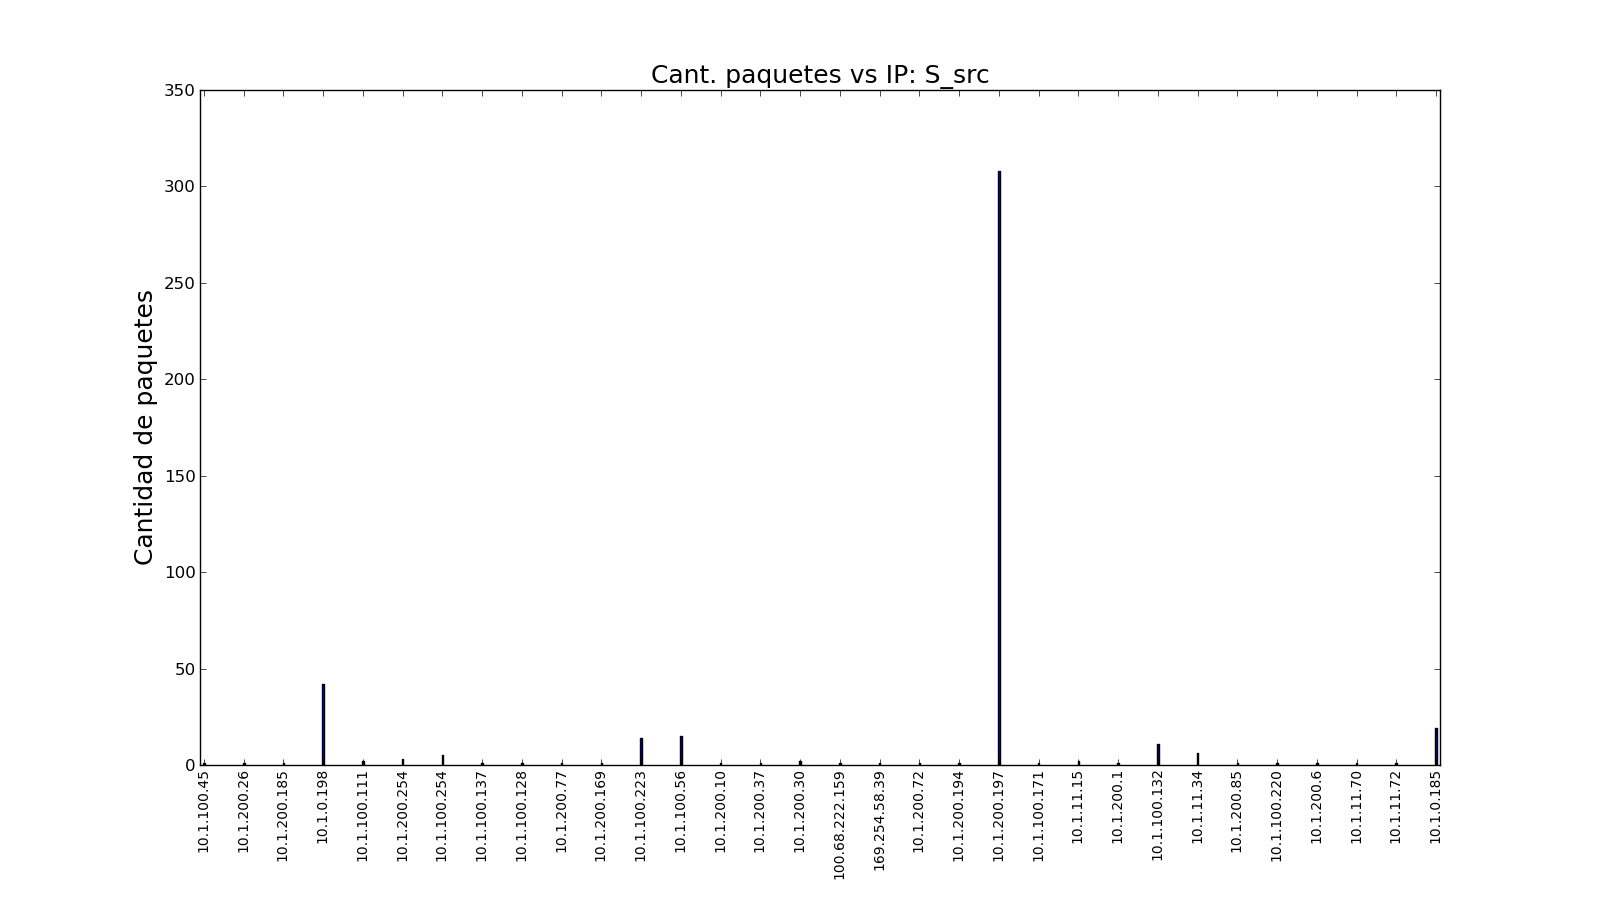
\includegraphics[width=0.8\linewidth]{../imgs/red-entrepiso-dc_S_src_hist.png}
    \caption{Histograma de la serie de paquetes s\_src de la red \emph{Entrepiso-DC}.}
    \label{fig:histograma-entrepiso-dc-s-src-ejemplo}
  \end{center}
  \end{figure}
  
\subsection{Gráfico información}

  En cada red y para cada una de las fuentes ($S_{src}$, $S_{dst}$), realizamos un gráfico donde se muestra la información de la aparición de un determinado IP en la fuente. Además, graficamos una recta (en rojo) mostrando el valor de la entropía de la fuente, para comparar fácilmente la información de cada IP con la entropía de la fuente. Se muestra un ejemplo en la figura \ref{fig:informacion-entrepiso-dc-s-src-ejemplo}.
  
  \begin{figure}  
  \begin{center}
    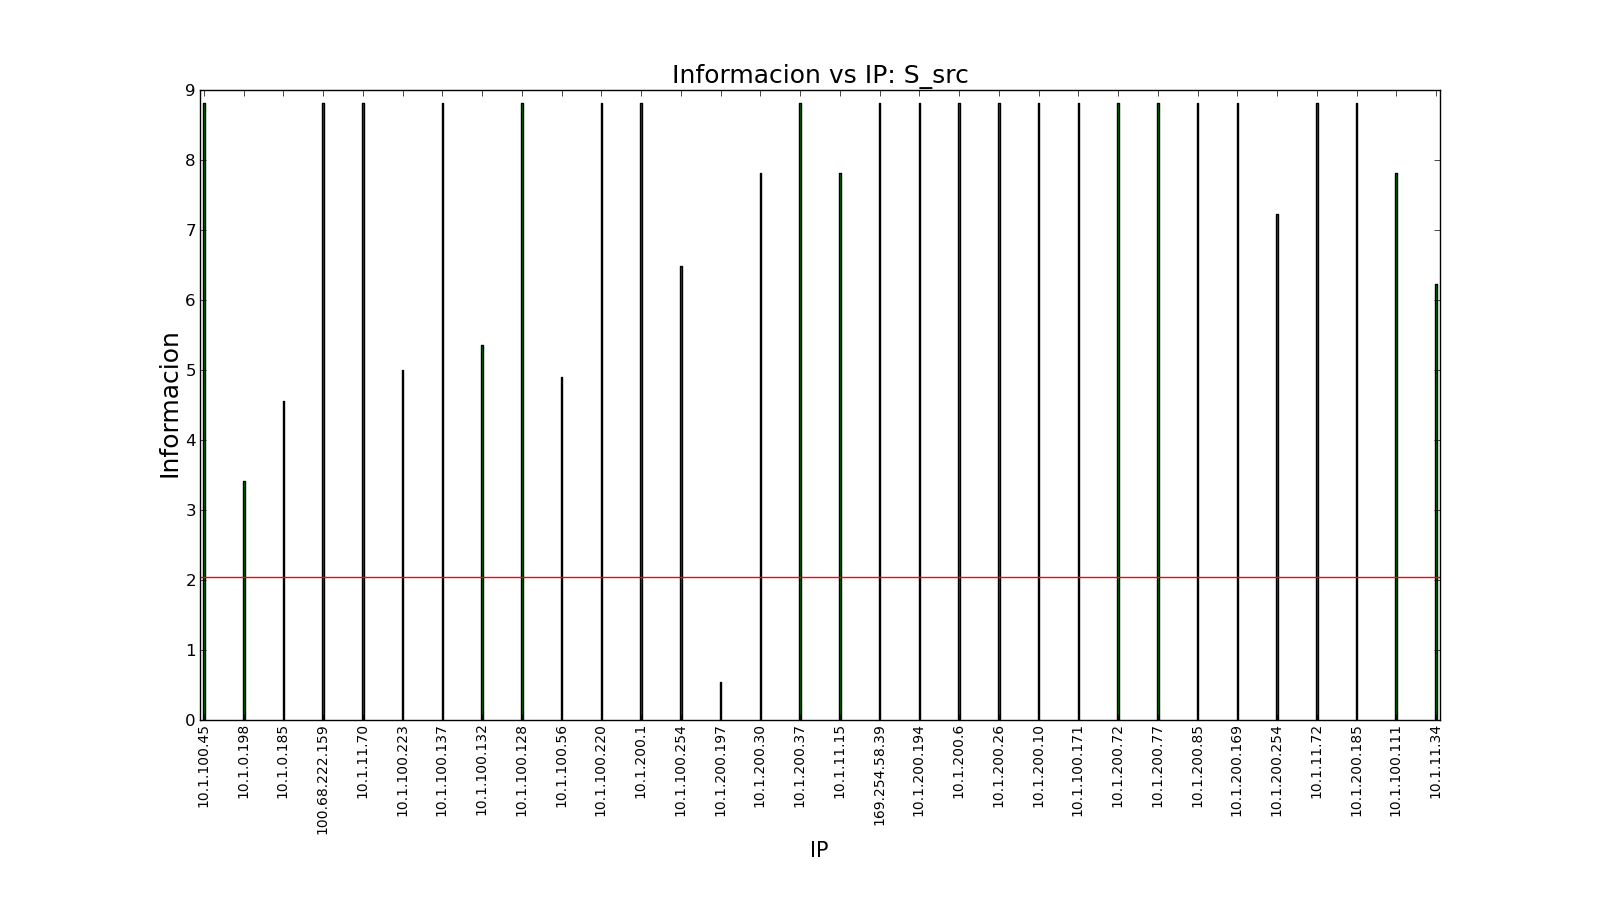
\includegraphics[width=0.8\linewidth]{../imgs/red-entrepiso-dc_S_src_info.png}
    \caption{Gráfico de cantidad de información para cada IP s\_src de la red \emph{Entrepiso-DC}.}
    \label{fig:informacion-entrepiso-dc-s-src-ejemplo}
  \end{center}
\end{figure}

\section{Resultados}

  \subsection{Red hogareña}
  \subsubsection{Descripción y grafo de relación entre los nodos}

En este primer experimento, capturamos el tráfico de la LAN de un integrante de nuestro grupo. Medimos un Miércoles a las 00:00hs utilizando la red Wi-Fi. El tiempo de medición fue de aproximadamente 40 minutos, y capturamos aproximadamente 20 paquetes.

\begin{figure}[H]
  \begin{center}
    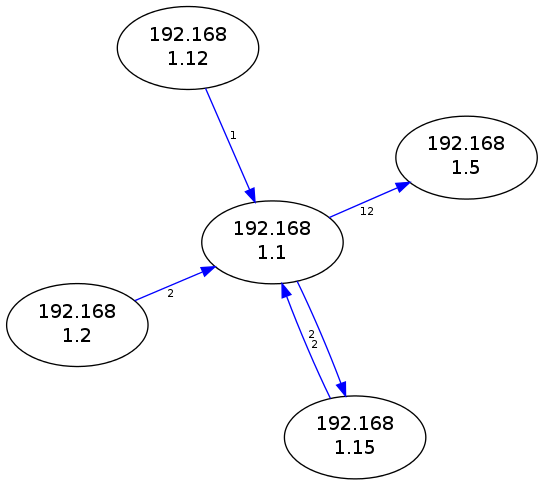
\includegraphics[width=0.3\linewidth]{../imgs/red-hogarena_red.png}
    \label{fig:FedeGrafo}
    \caption{Grafo de LAN hogareña}
  \end{center}
\end{figure}

\subsubsection{Fuente: $S_{dst}$}

\begin{figure}[H]\centering
    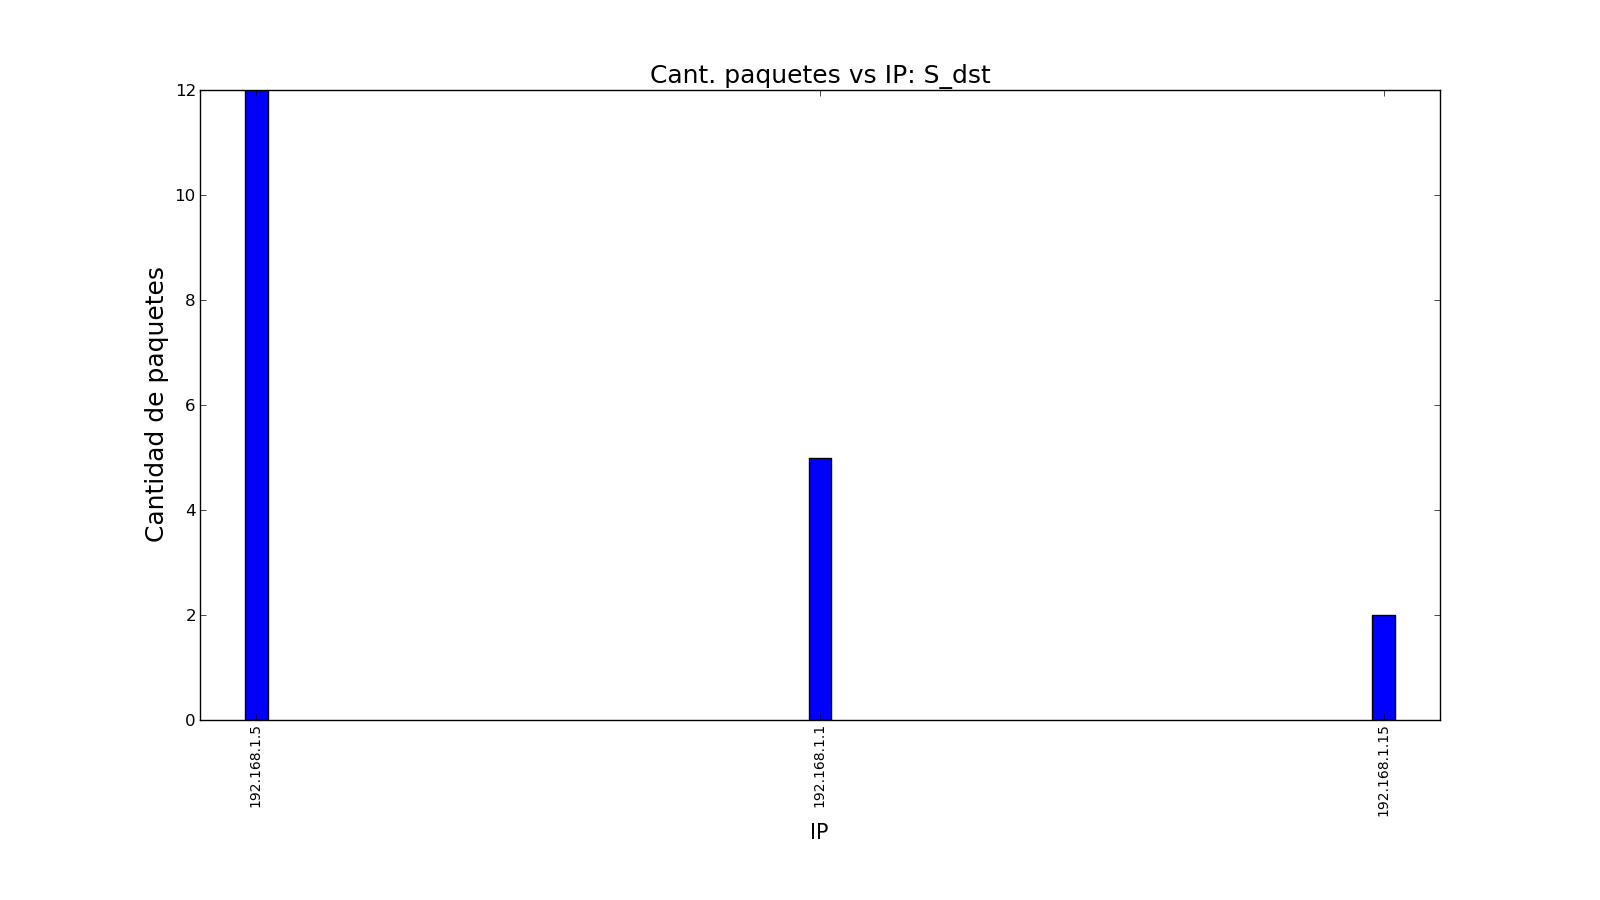
\includegraphics[width=0.8\linewidth]{../imgs/red-hogarena_S_dst_hist.png}
    \caption{Histograma de $S_{dst}$}\label{fig:Fede-dst-hist}
\end{figure}

\begin{figure}[H]\centering
    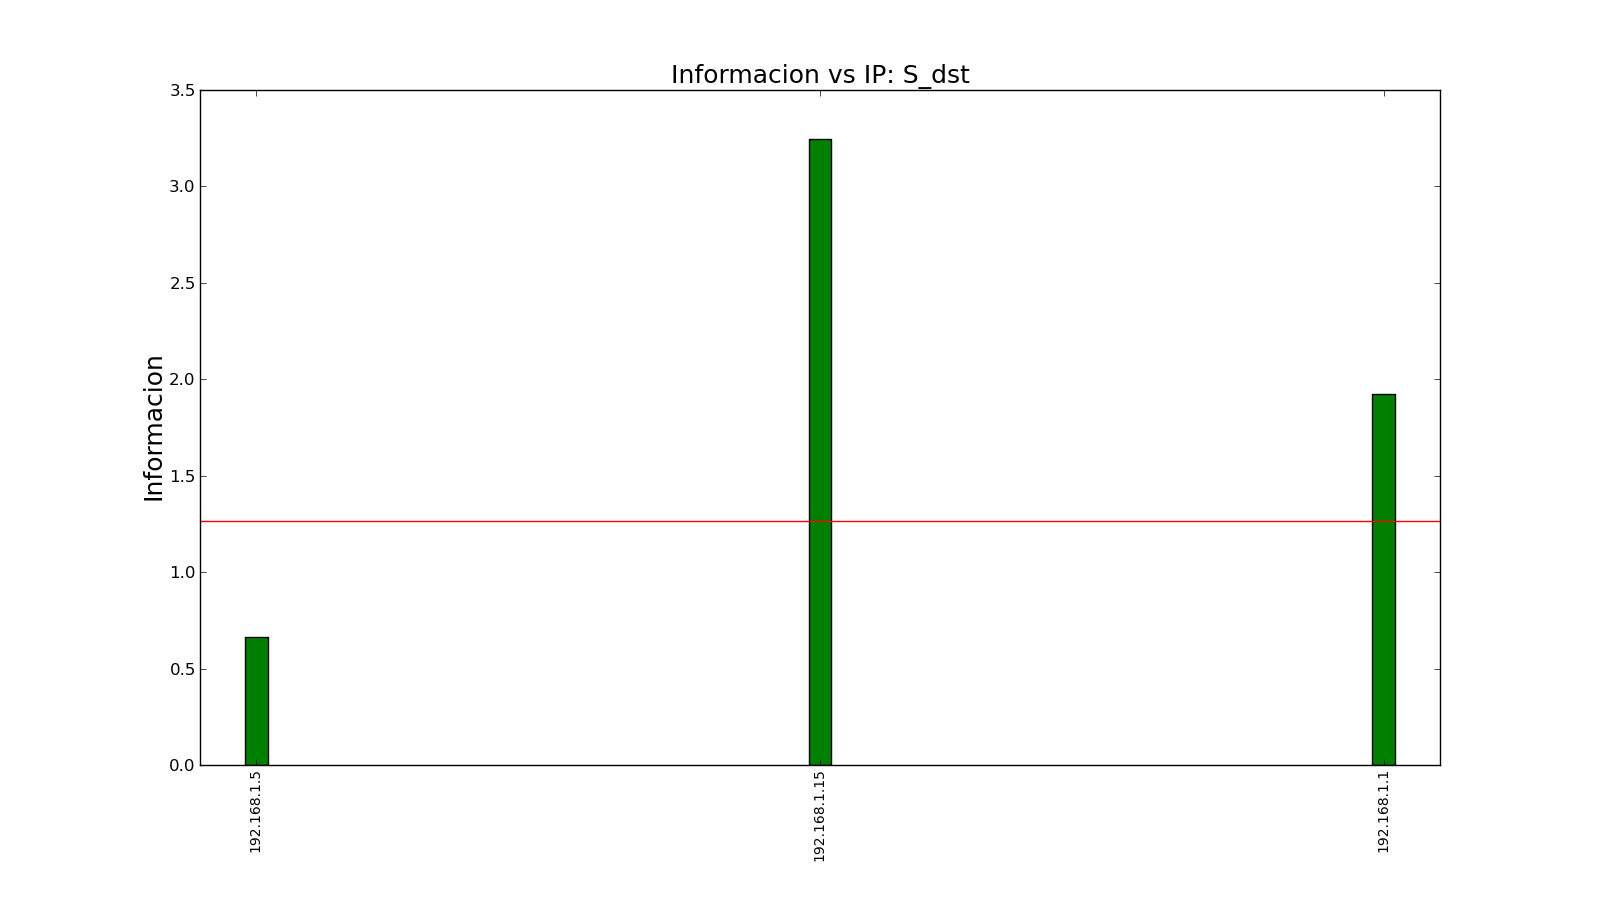
\includegraphics[width=0.8\linewidth]{../imgs/red-hogarena_S_dst_info.png}
    \caption{Informacion de $S_{dst}$}\label{fig:Fede-dst-info}
\end{figure}

$\bullet$ Entropía de la fuente: 1.26744380381

\subsubsection{Fuente: $S_{src}$}

\begin{figure}[H]\centering
    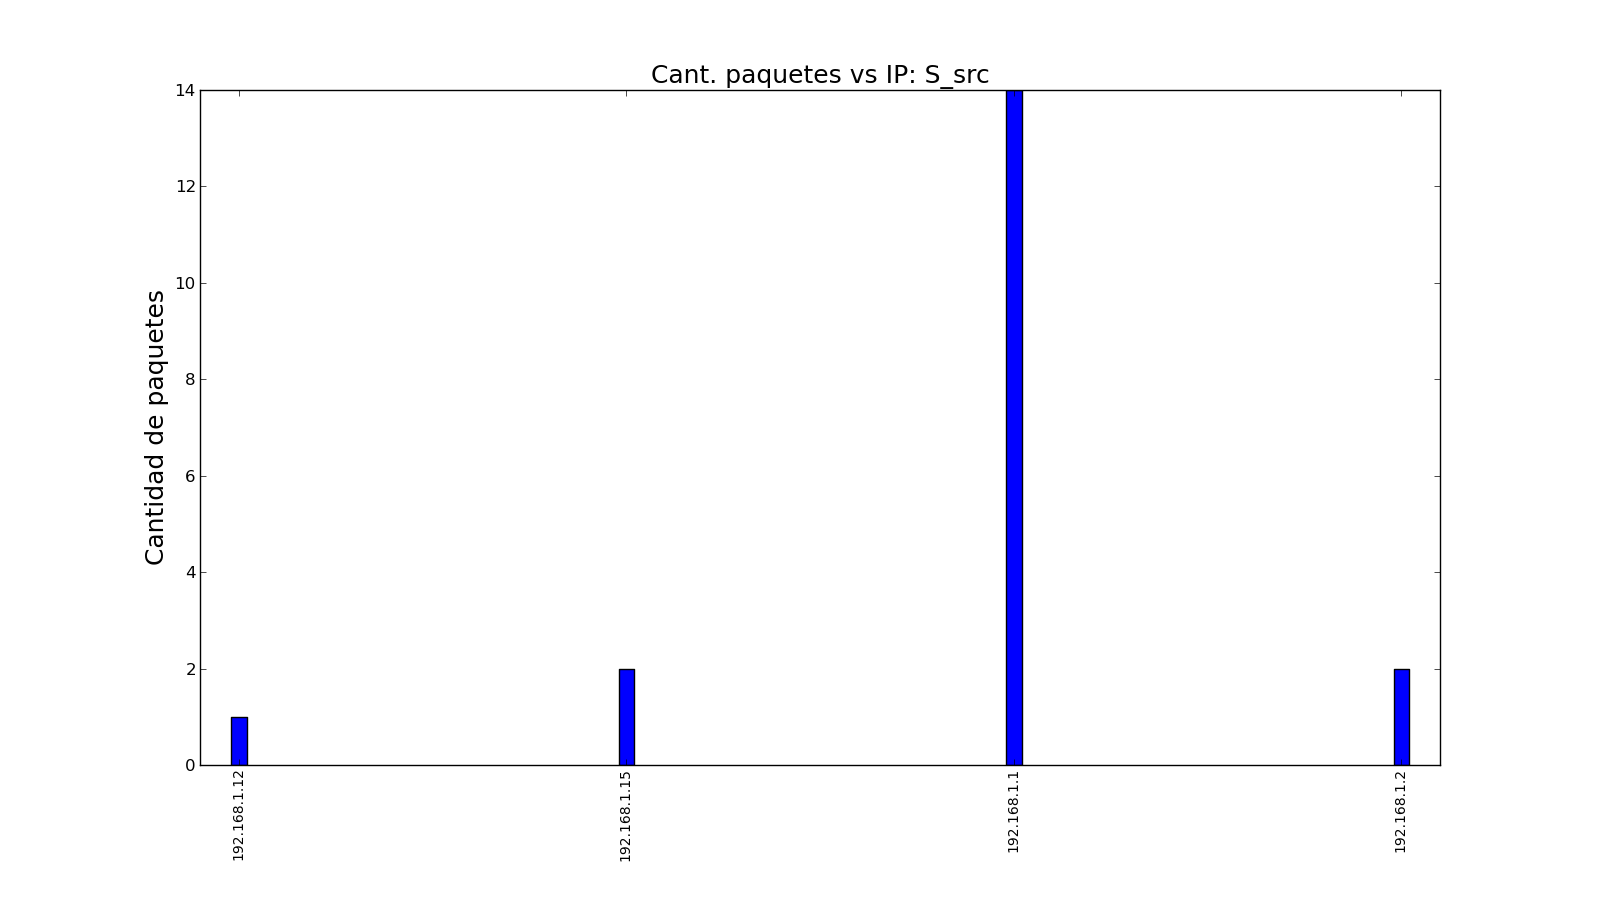
\includegraphics[width=0.8\linewidth]{../imgs/red-hogarena_S_src_hist.png}
    \caption{Histograma de $S_{src}$}\label{fig:Fede-src-hist}
\end{figure}

\begin{figure}[H]\centering
    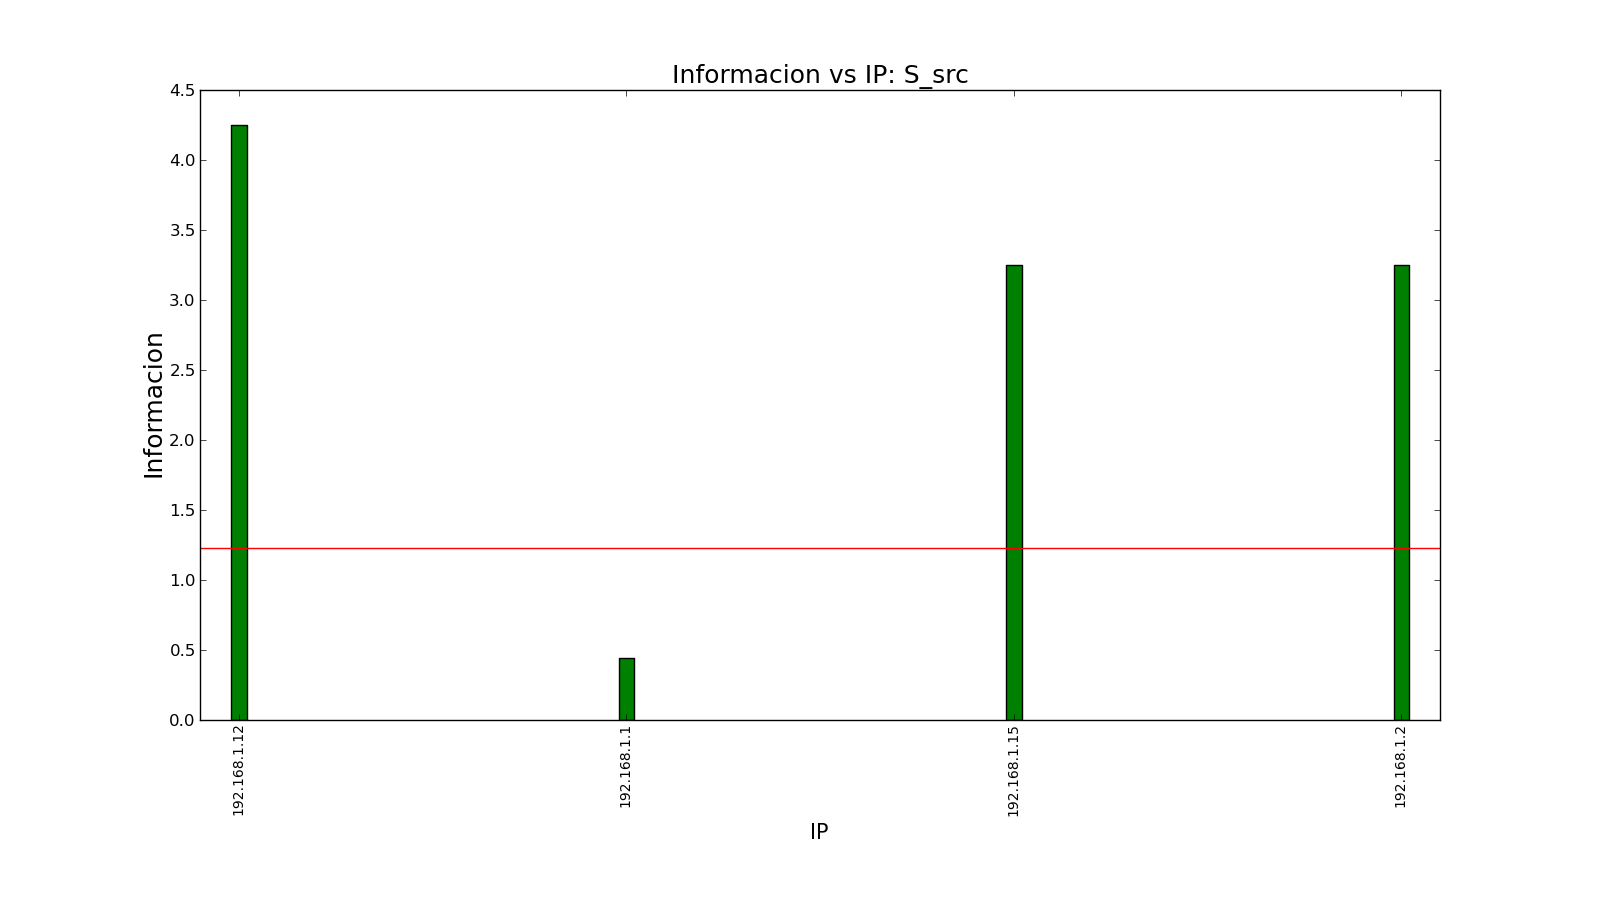
\includegraphics[width=0.8\linewidth]{../imgs/red-hogarena_S_src_info.png}
    \caption{Informacion de $S_{src}$}\label{fig:Fede-src-info}
\end{figure}

$\bullet$ Entropía de la fuente: 1.2319817814

\subsubsection{Discusión}

Debido a que es una red hogareña, tenemos una red bastante chica. En el grafo podemos observar un nodo (\emph{192.168.1.1}) el cual se conecta con todos los demás. A esta red la conocemos, y sabemos que dicho nodo es el router.

Como podemos observar en la Figura \ref{fig:Fede-src-info}, el router es un nodo distinguido en la fuente $S_{src}$. Sin embargo, en la Figura \ref{fig:Fede-dst-info} (fuente $S_{dst}$) el único nodo distinguido es \emph{192.168.1.5}. En el caso de \emph{192.168.1.5}, es una computadora que estaba bajando un archivo .torrent, y creemos que por eso 12 paquetes ARP \emph{who-has} tienen destino \emph{192.168.1.5}.

  \subsection{Red Alto Palermo}
  \subsubsection{Descripción y topología de los paquetes}

Nuestro primer experimento consistió en medir la LAN Wi-Fi pública del shopping Alto Palermo. Esta medición se llevó a cabo el Sábado 20 de Septiembre a las 21hs, el tiempo de medición fue de aproximádamente 40 minutos y se capturaron 1569 paquetes ARP.

Sin embargo, para graficar decidimos usar sólo los primeros 80 paquetes capturados, ya que los graficos con una cantidad tan grande de paquetes eran poco legibles.

A continuación mostramos un grafo que muestra los nodos de la red con su dirección IP y la cantidad de mensajes de tipo \emph{who-has}.

\begin{figure}[H]
 \begin{center}
  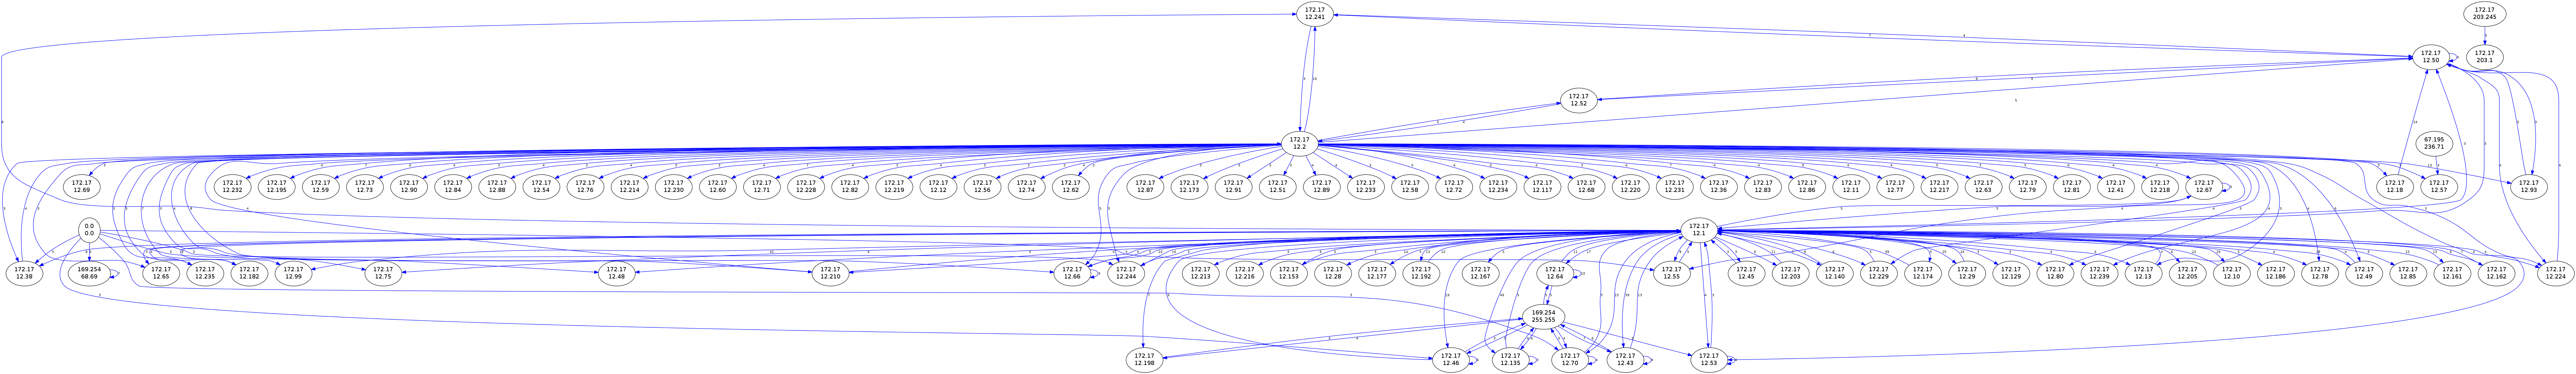
\includegraphics[width=\linewidth]{../imgs/snifAlto-ips_red.png}
  \caption{Grafo Medición Alto Palermo}
 \end{center}

\end{figure}

Como podemos ver en el grafo, la red tiene dos nodos que se destacan. Uno de estos nodos, el cual tiene la dirección IP 117.17.12.1, recibe muchos paquetes de la mayoría de los otros nodos de la red, pero no envía ninguno. Y el otro recibe varios paquetes y también envía varios.

\subsubsection{Fuente: $S_{dst}$}

A continuación incluimos dos gráficos. Uno de éstos es un histograma que muestra cuántas veces apareció cada símbolo en la fuente. El otro, muestra la cantidad de información de cada símbolo de la fuente $S_{dst}$ en comparación con la entropía de la misma. 

\begin{figure}[H]
   \begin{minipage}{0.5\linewidth}
     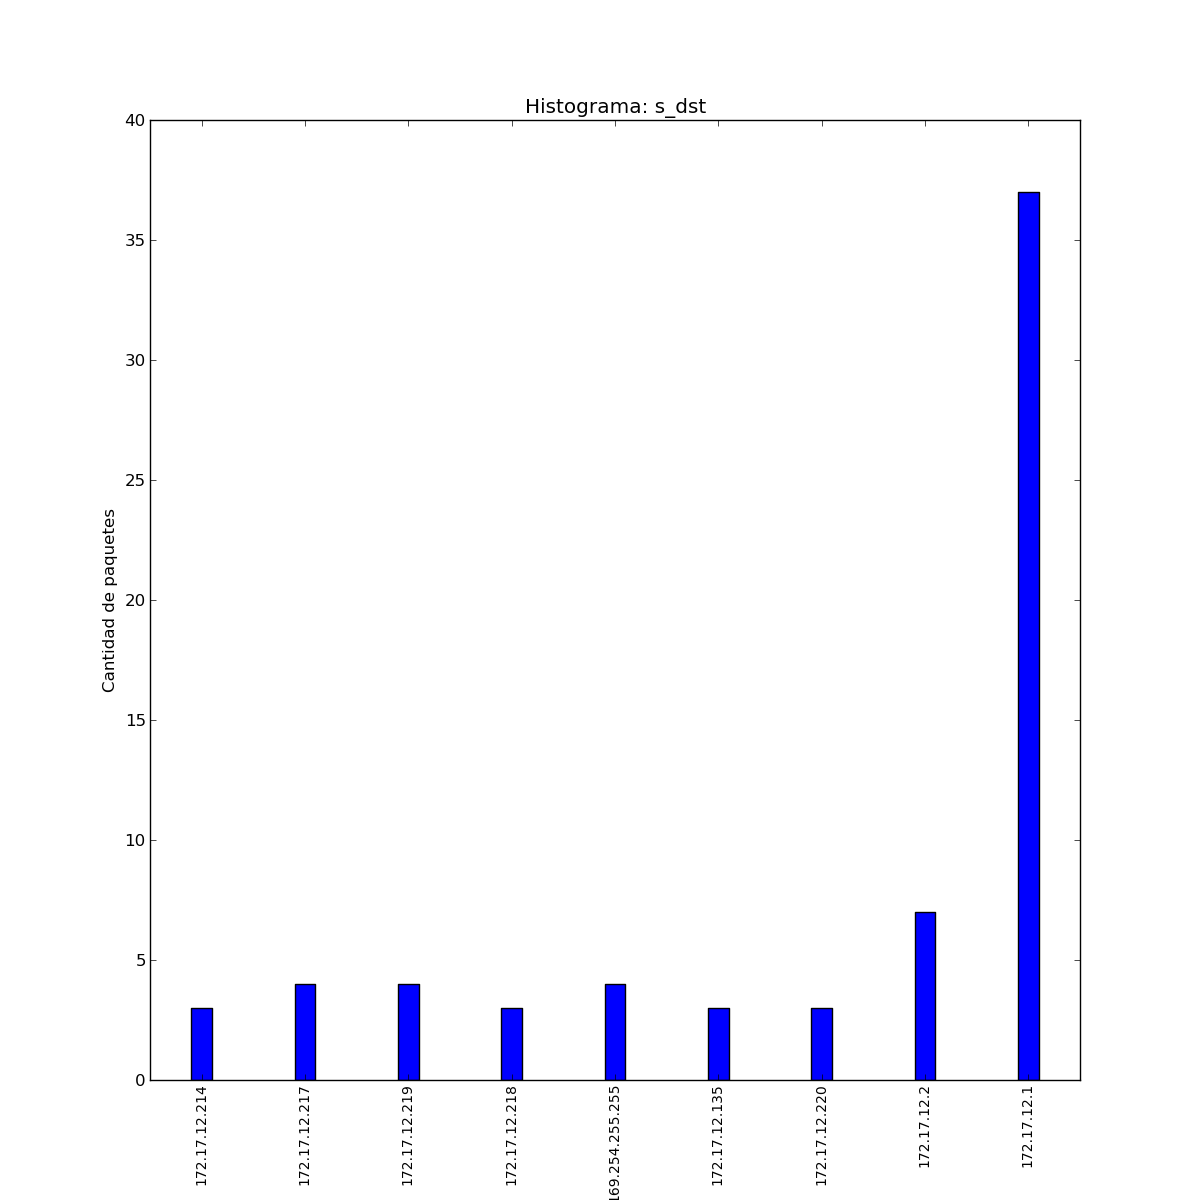
\includegraphics[width=\linewidth]{../imgs/snifAlto-ips_s_dst_hist.png}
     \caption{Medición Alto Palermo}\label{fig:Alto-dst-hist}
   \end{minipage}
  \hfill
   \begin{minipage}{0.5\linewidth}
     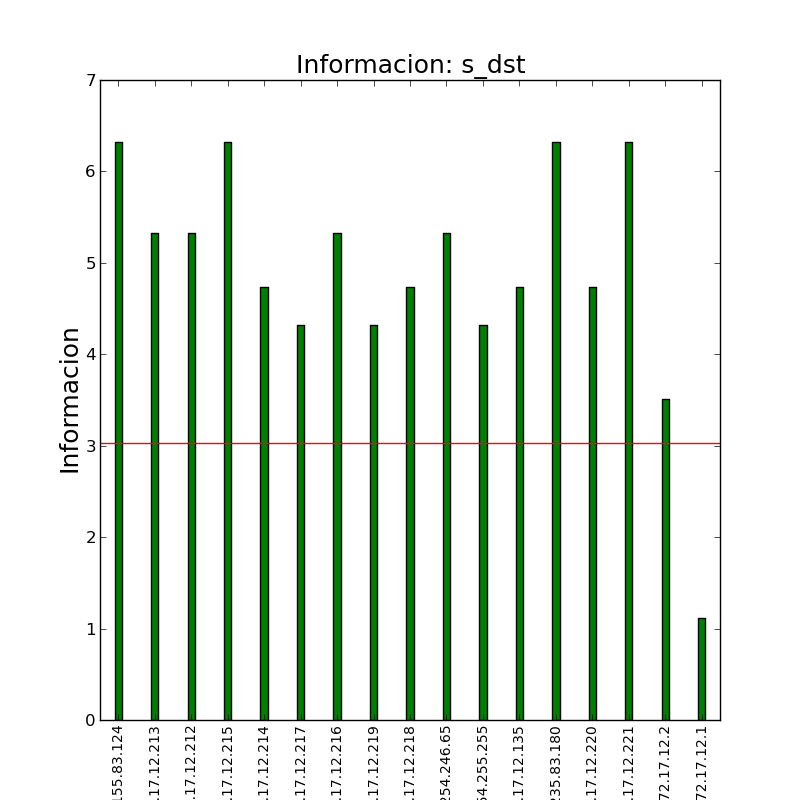
\includegraphics[width=\linewidth]{../imgs/snifAlto-ips_s_dst_info.png}
     \caption{Medición Información Alto Palermo}\label{fig:Alto-dst-info}
   \end{minipage}
 \end{figure}

Como podemos observar en el primer gráfico, la dirección IP 177.17.12.1 aparece muchas más veces que el resto de las IP. Esto es así porque dicha dirección recibe mensajes de casi todos los demás nodos de la red.

En el segundo gráfico podemos ver que la cantidad de información que aporta la dirección IP 177.17.12.1 es más baja que la entopía de la fuente.
 
 
\subsubsection{Fuente: $S_{src}$}

A contincuación mostramos gráficos similares, pero esta vez para la fuente $S_{src}$:

\begin{figure}[H]
   \begin{minipage}{0.5\linewidth}
     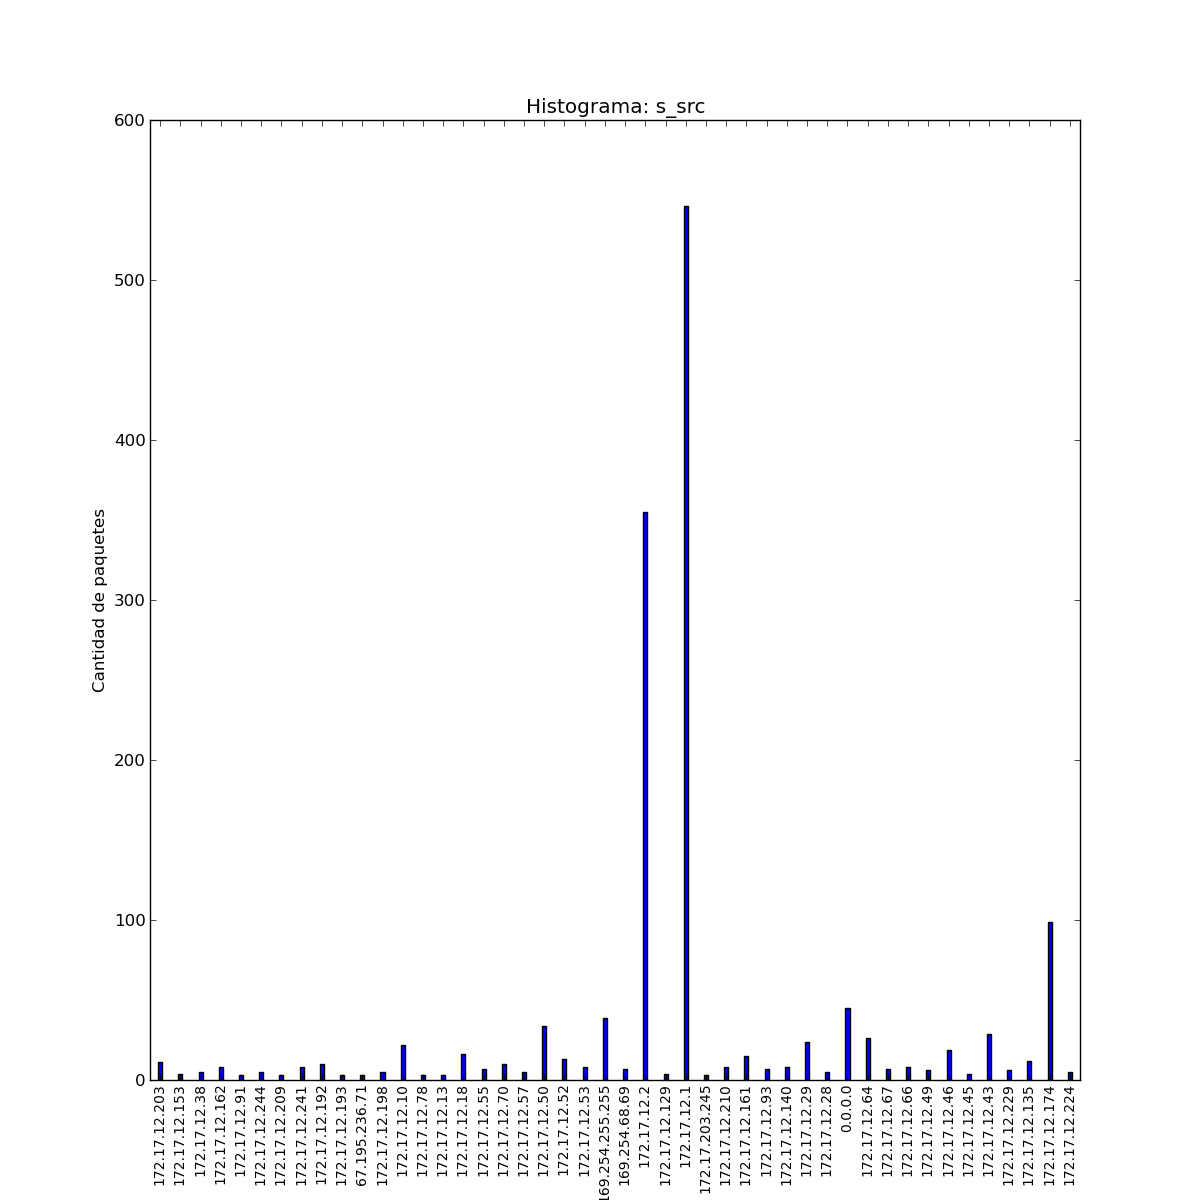
\includegraphics[width=\linewidth]{../imgs/snifAlto-ips_s_src_hist.png}
     \caption{Medición Honeywell}\label{fig:Alto-src-hist}
   \end{minipage}
  \hfill
   \begin{minipage}{0.5\linewidth}
     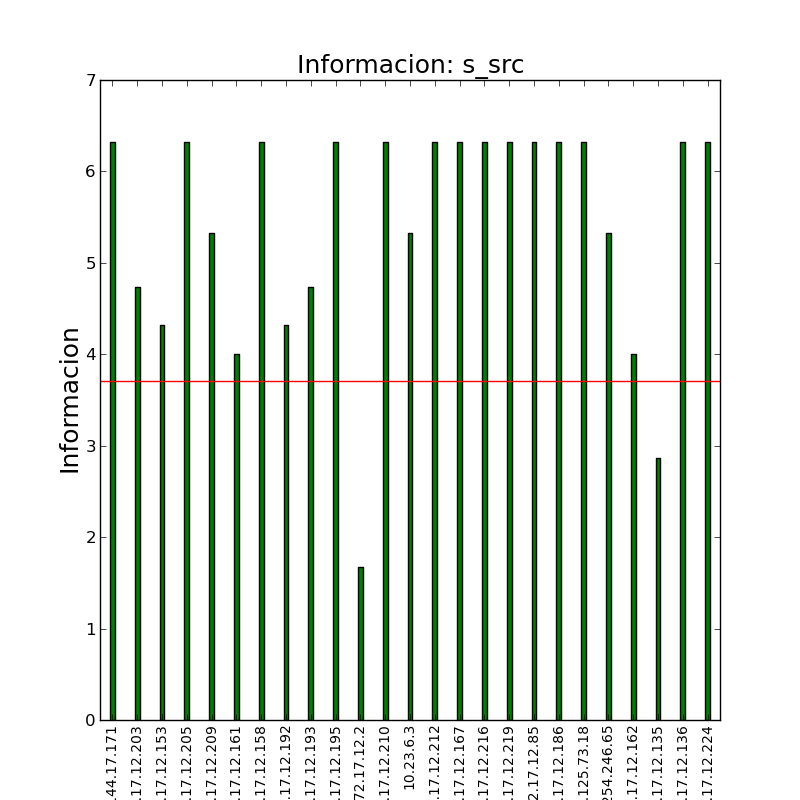
\includegraphics[width=\linewidth]{../imgs/snifAlto-ips_s_src_info.png}
     \caption{Medición Honeywell}\label{fig:Alto-src-info}
   \end{minipage}
 \end{figure}

En estos gráficos podemos observar que hay un nodo que envía muchos más paquetes que el resto de los nodos. Dicho nodo tiene la dirección IP 172.17.12.2. En el segundo gráfico podemos observar que la cantidad de información del símbolo 172.17.12.2 en la fuente $S_{src}$ es menor que su entropía.

Además podemos ver que hay otro nodo distinguido en esta fuente, el nodo que tiene la IP 172.17.12.135. Sin embargo, podemos ver que este nodo manda menos paquetes que el nodo 172.17.12.2.
 
\subsubsection{Discusión}

Cuando observamos el grafo en la primera parte del análisis de esta red, dijimos que había dos nodos que se destacaban visualmente, los cuales eran los que tenían las direcciones IP 177.17.12.1 y 177.17.12.2. Al ver el grafo notamos que la mayor parte de los paquetes capturados eran enviados o recibidos por alguno de estos dos nodos. Esto nos hizo suponer que éstos eran los dos nodos distinguidos de la red.

Al luego observamos el histograma y el gráfico de barras de la fuente $S_{dst}$. De esta forma vimos que efectivamente el nodo con la IP 117.17.12.1 aparecía como dirección destino en muchos mensajes. Sin embargo el nodo 177.17.12.2 no aparecía tantaas veces.

Luego de hacer lo mismo con la fuente $S_{src}$ notamos que el nodo que aparecía más veces era el nodo 177.17.12.2. El nodo 177.17.12.1 no era un símbolo de $S_{src}$ ya que éste no mando mensajes, por lo tanto no aparece en estos gráficos.

Concluimos entonces que el nodo de la red que tiene la dirección IP 177.17.12.1 se trata de un nodo distinguido, el cual creemos que es el router de la red. Sin embargo, no pudimos ver qué rol ocupaba el nodo 177.17.12.2 en la misma.

  \subsection{Red Honeywell}
  \subsubsection{Descripción y grafo de relación entre los nodos}

Nuestro segundo experimento consistió en capturar los paquetes de la LAN Wi-Fi de la empresa Honeywell. En esta red no hay mucho tráfico, ya que la mayoría de las computadores se conectan via Ethernet a una VPN. Esta red es dedicada a transacciones que no necesiten un nivel de seguridad. La captura se realizo un día lunes a las 11 am. durante media hora, lográndose capturar 253 paquetes.  

\begin{figure}[H]
 \begin{center}
  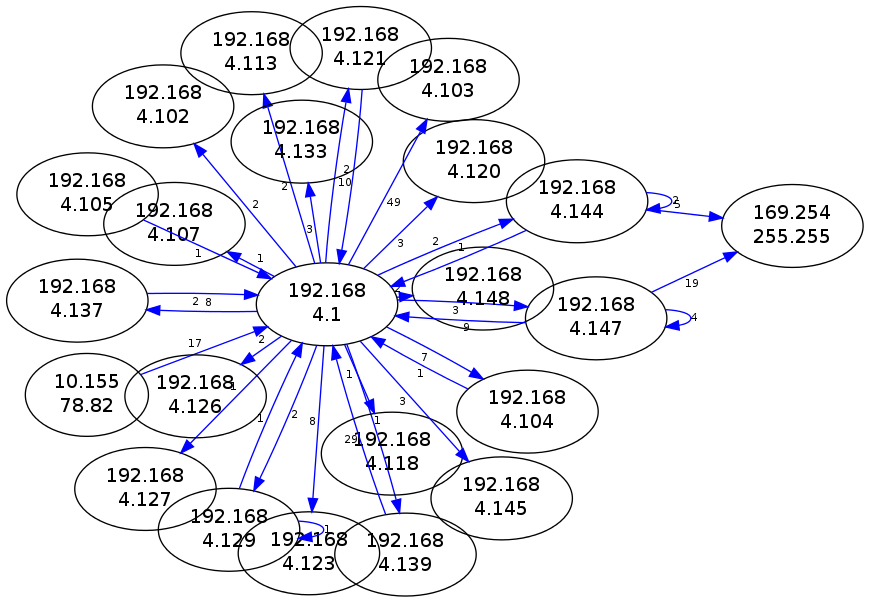
\includegraphics[width=0.7\linewidth]{../imgs/red-honeywell_red.png}
  \caption{Medición Honeywell}
 \end{center}
\end{figure}


\subsubsection{Fuente}

\begin{figure}[H]\centering
    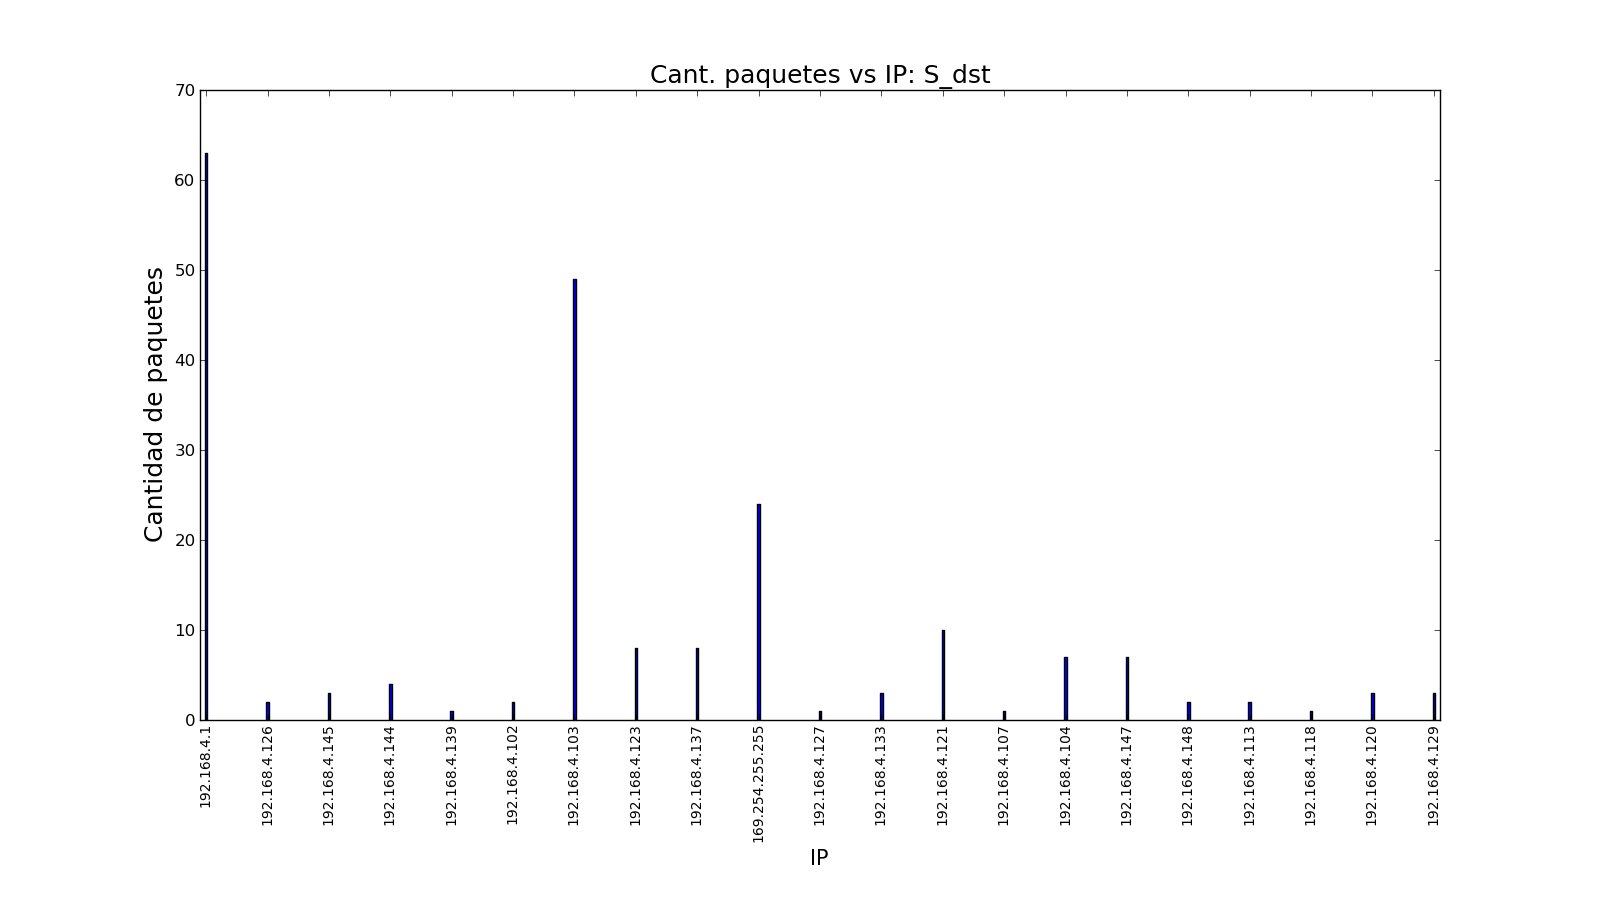
\includegraphics[width=0.8\linewidth]{../imgs/red-honeywell_S_dst_hist.png}
    \caption{Histograma de $S_{dst}$}\label{fig:Honeywell-dst-hist}
\end{figure}

\begin{figure}[H]\centering
    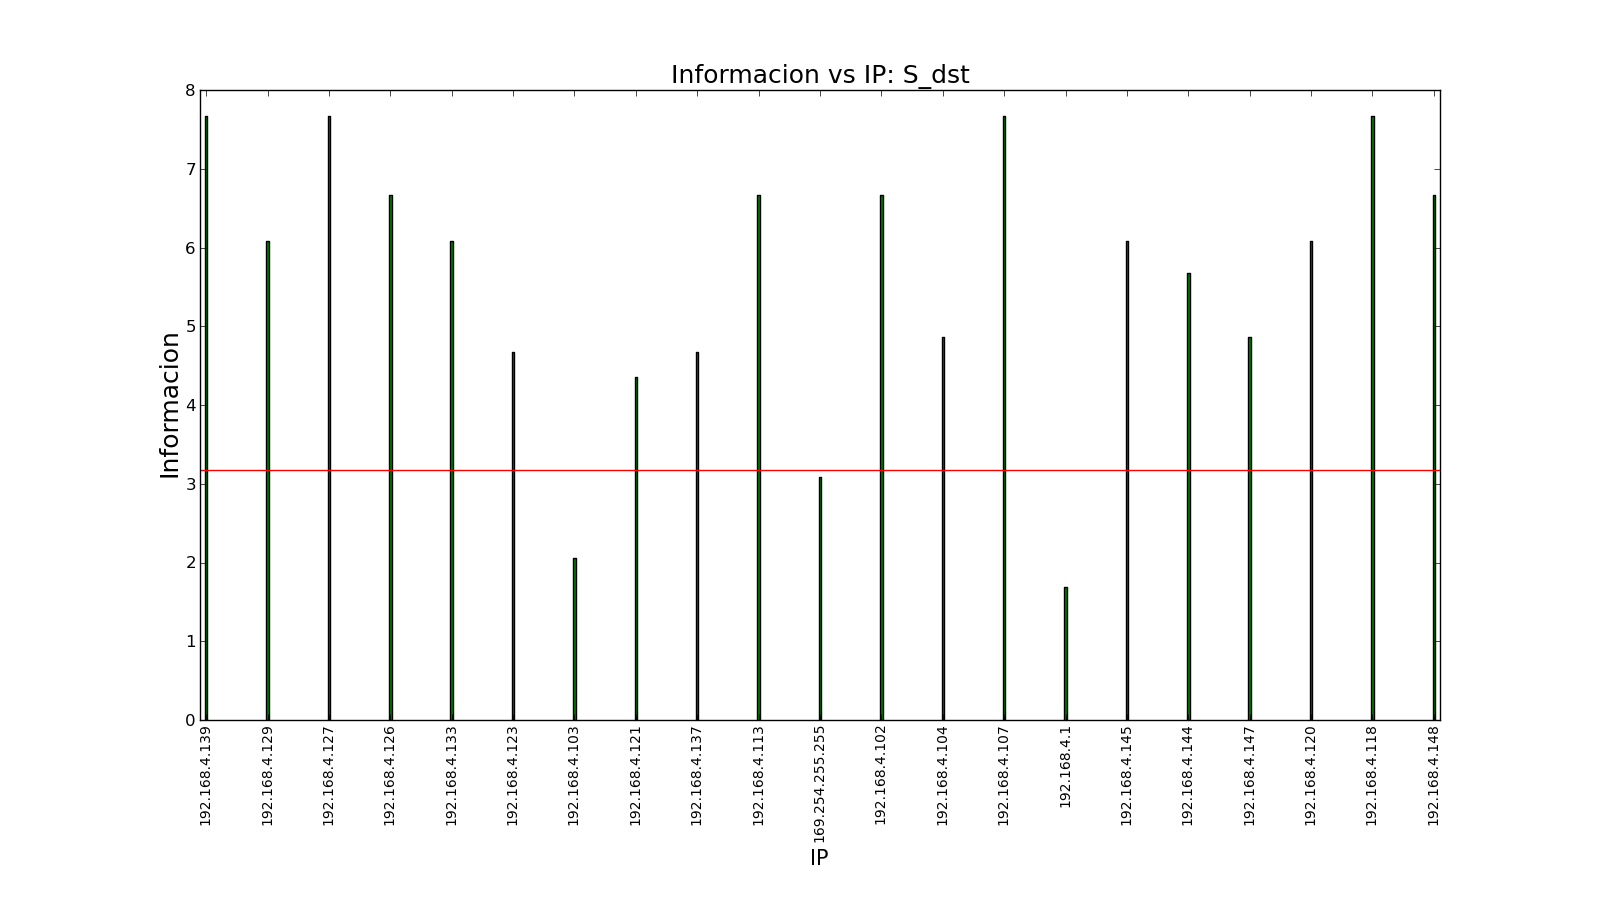
\includegraphics[width=0.8\linewidth]{../imgs/red-honeywell_S_dst_info.png}
    \caption{Informacion de $S_{dst}$}\label{fig:Honeywell-dst-info}
\end{figure}

$\bullet$ Entropía de la fuente: 3.17600221734

\subsubsection{Fuente: $S_{src}$}

\begin{figure}[H]\centering
    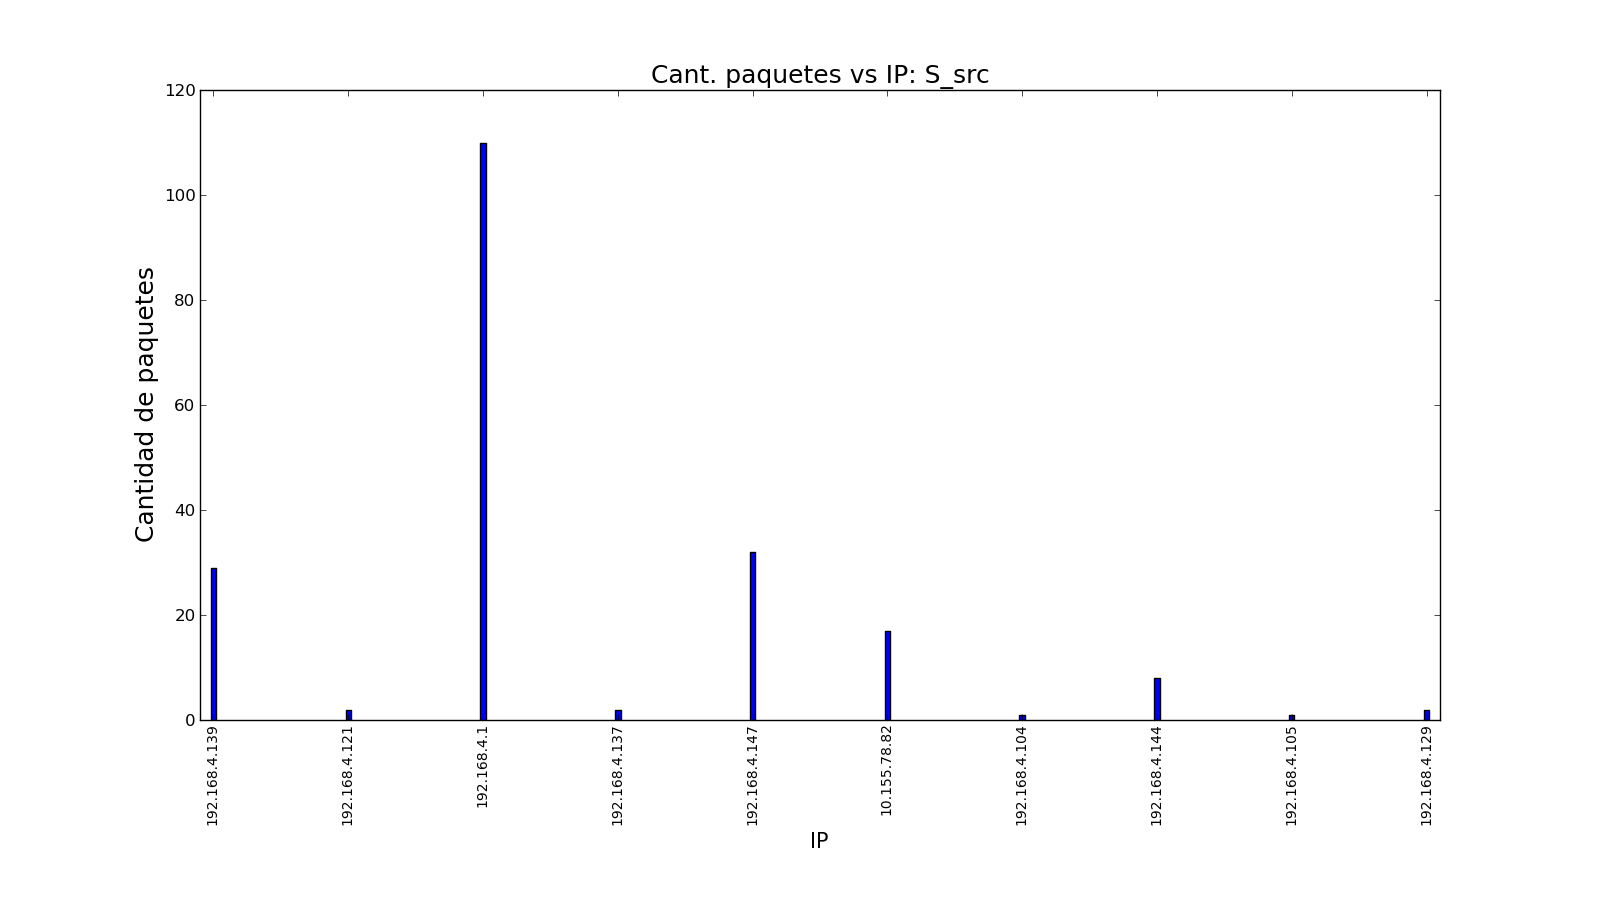
\includegraphics[width=0.8\linewidth]{../imgs/red-honeywell_S_src_hist.png}
    \caption{Histograma de $S_{src}$}\label{fig:Honeywell-src-hist}
\end{figure}

\begin{figure}[H]\centering
    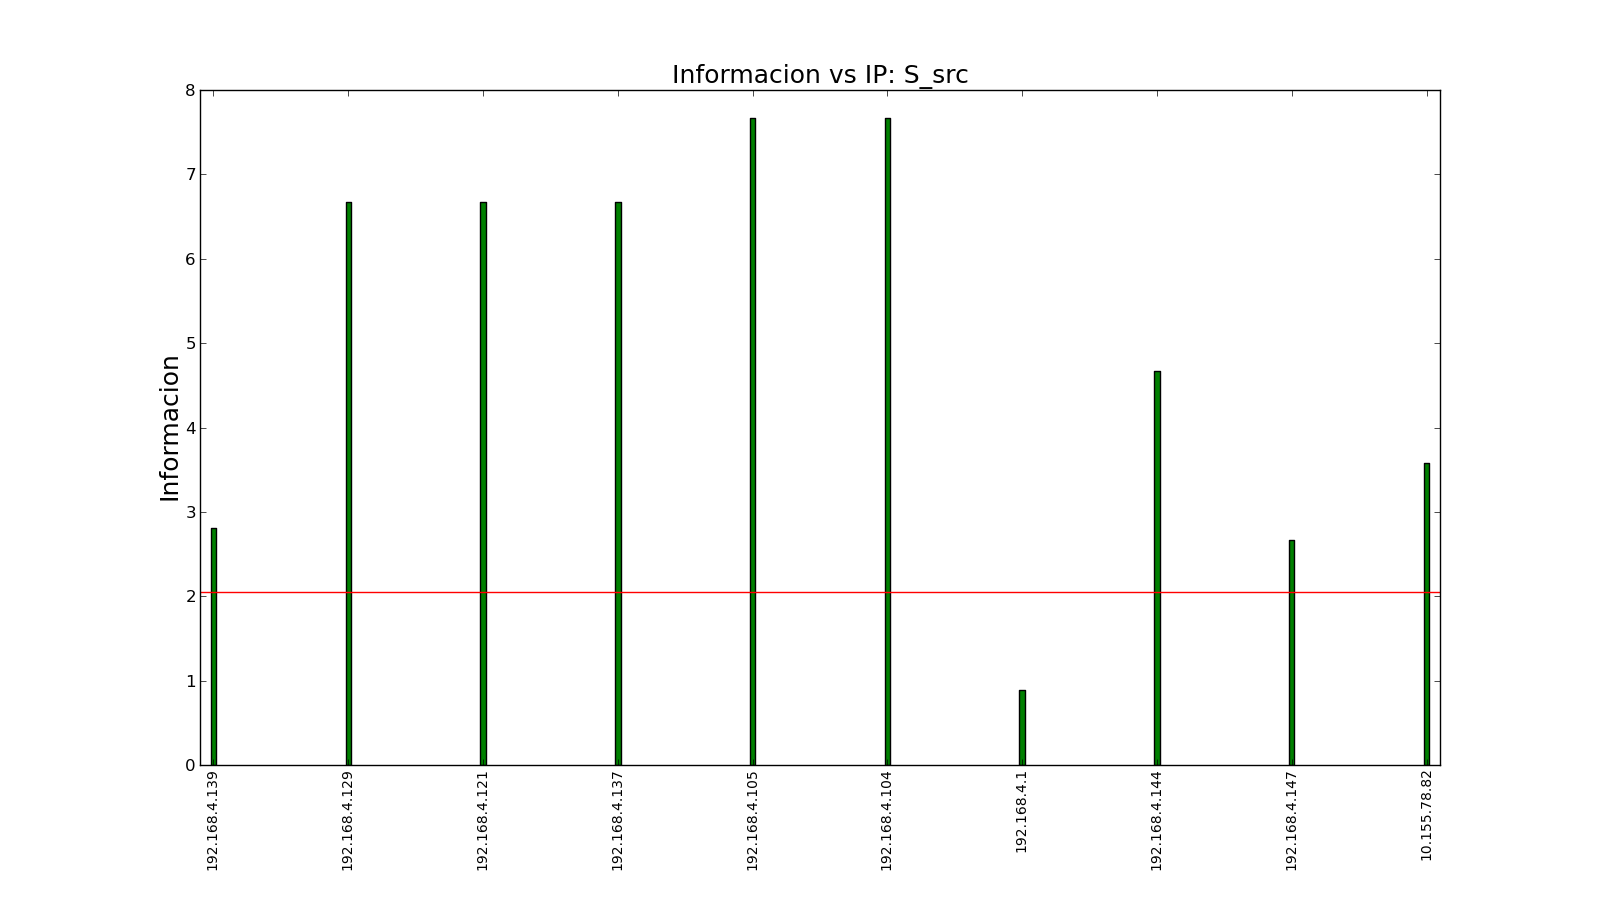
\includegraphics[width=0.8\linewidth]{../imgs/red-honeywell_S_src_info.png}
    \caption{Informacion de $S_{src}$}\label{fig:Honeywell-src-info}
\end{figure}

$\bullet$ Entropía de la fuente: 2.05322002017

\subsubsection{Discusión}

cualquier cosa interesante sobre este caso en particular

  \subsection{Red Laboratorios DC}
  \subsubsection{Descripción y topología de los paquetes}

Realizamos una captura en la red Wi-Fi \emph{Entrepiso-DC}, disponible desde los laboratorios del Depto. de Computación. La muestra fue tomada un lunes a las 17hs aproximadamente -horario típicamente de alto tráfico-, logrando un total de XX paquetes en MM minutos.

En el gráfico de la figura \ref{fig:entrepiso-dc-grafo} se presenta el grafo dirigido representando la red. En el mismo se observa una gran cantidad de nodos ligada al nodo con IP 10.1.200.197, y luego múltiples conjuntos pequeños de nodos conectados entre sí pero disconexos de la estructura mayoritaria.

\begin{figure}[H]
  \begin{center}
    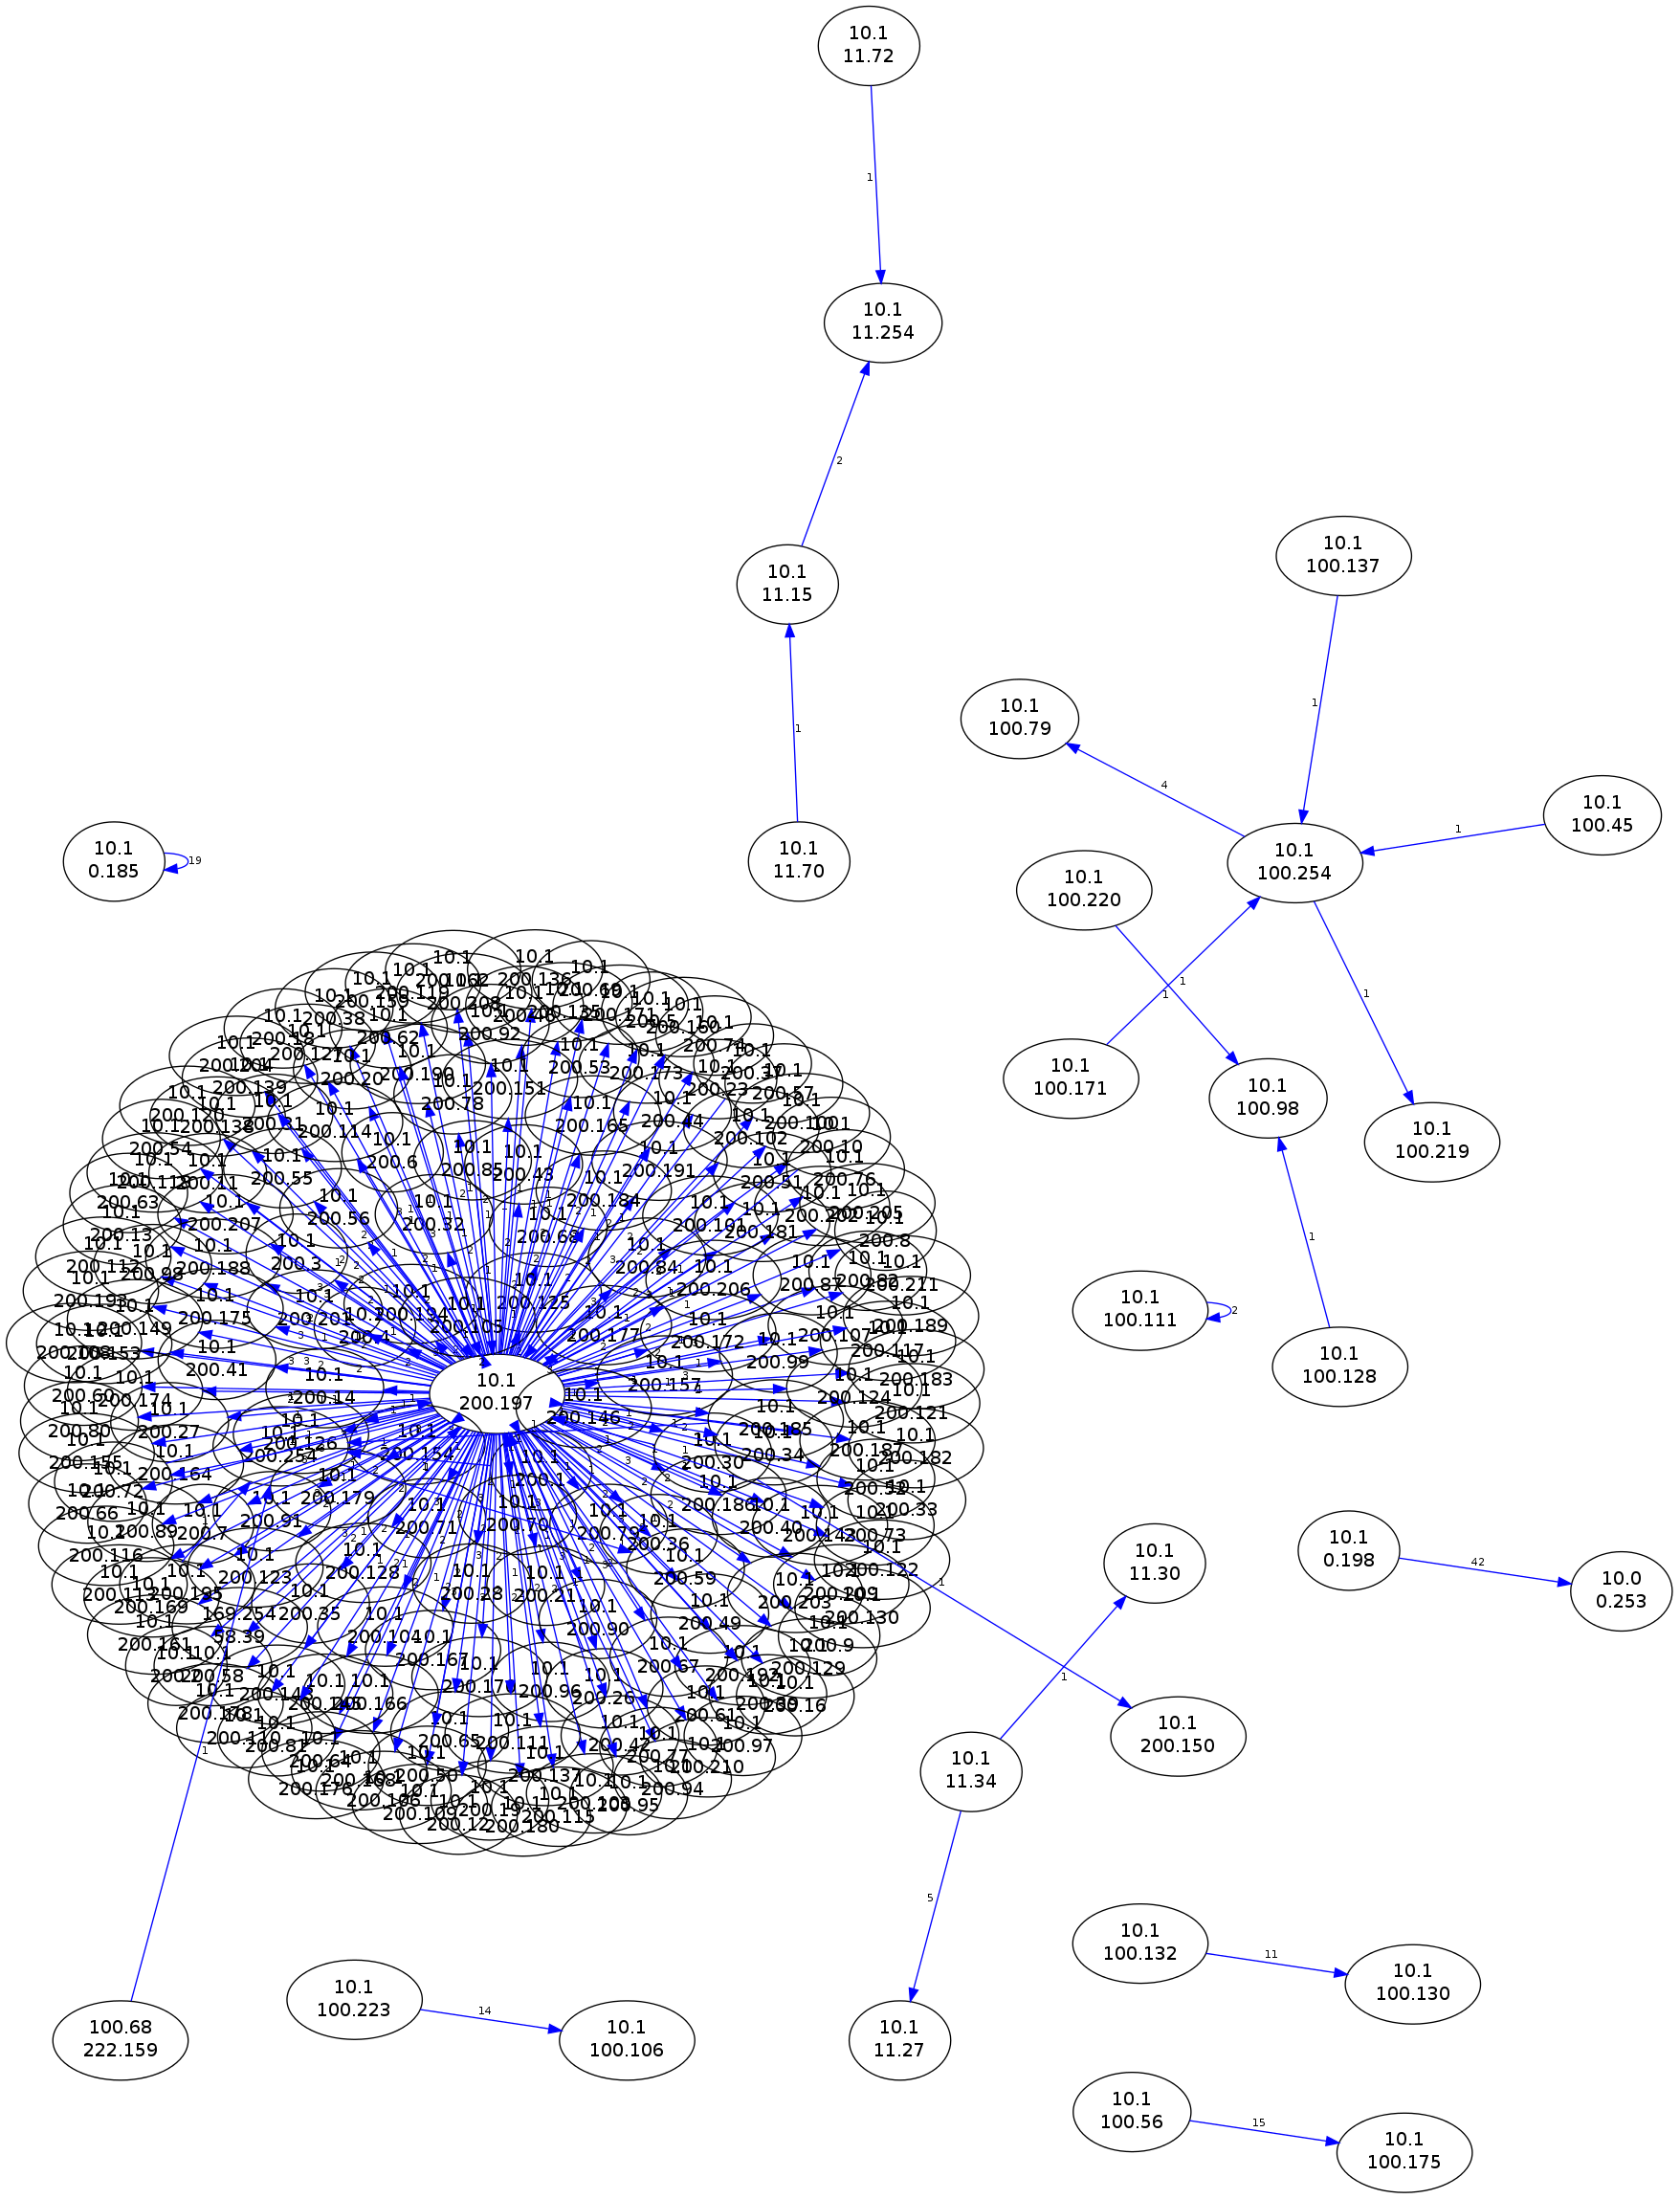
\includegraphics[width=0.6\linewidth]{../imgs/red-entrepiso-dc_red.png}
    \caption{Grafo mostrando la topología de la red \emph{Entrepiso-DC}.}
    \label{fig:entrepiso-dc-grafo}
  \end{center}
\end{figure}

\subsubsection{Fuente: $S_{dst}$}

\begin{figure}[H]\centering
    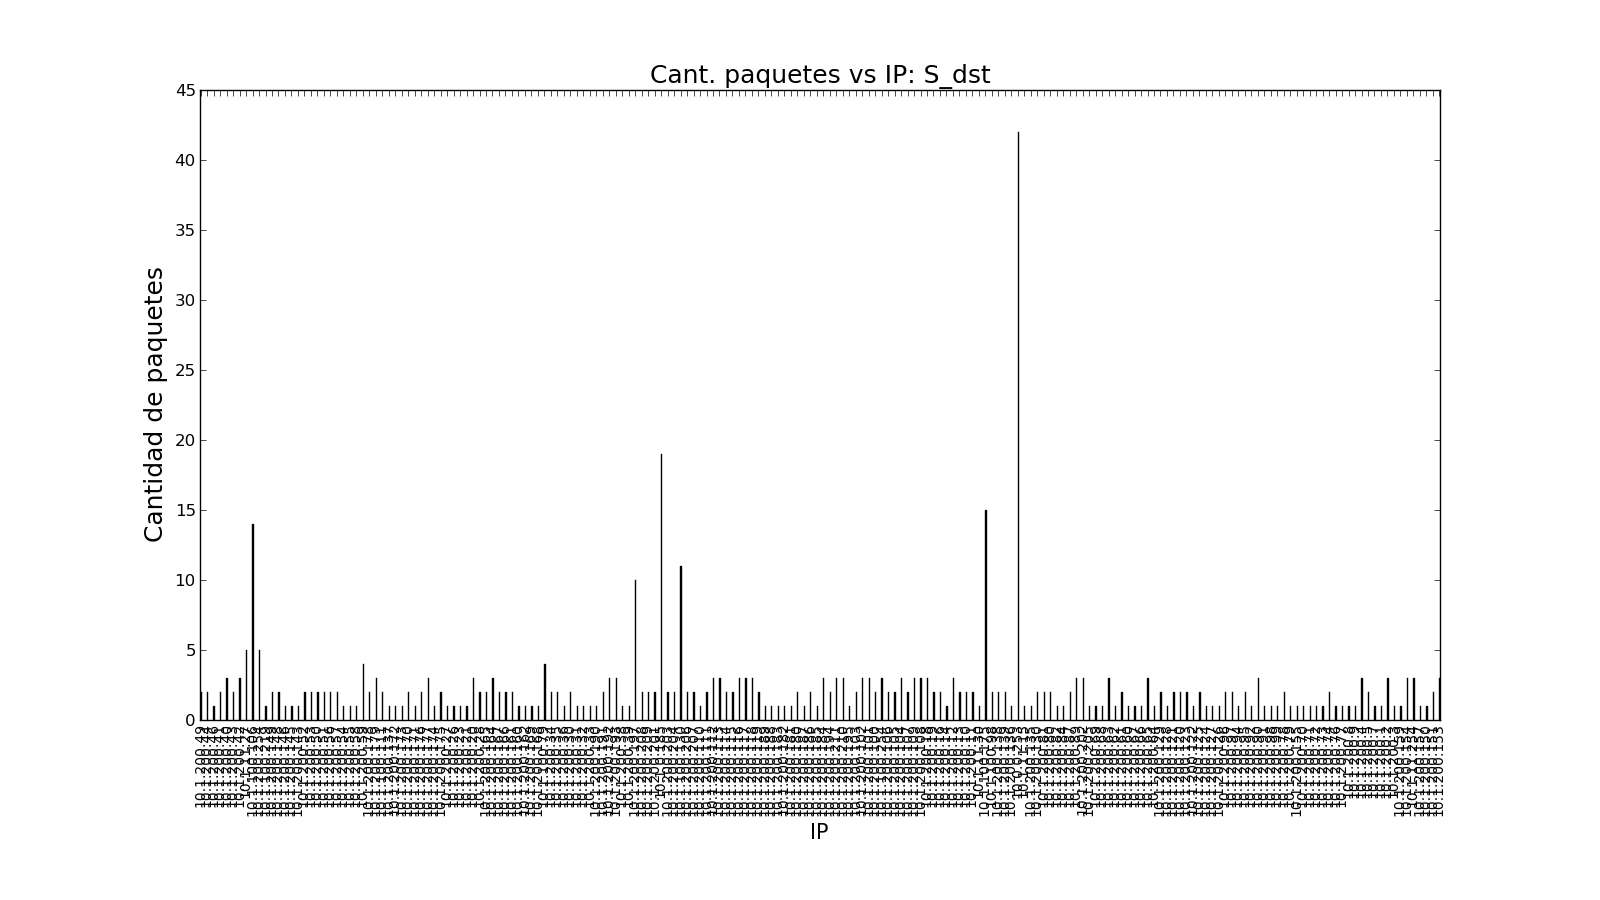
\includegraphics[width=\linewidth]{../imgs/red-entrepiso-dc_S_dst_hist.png}
    \caption{Histograma de $S_{dst}$}\label{fig:entrepiso-dc-dst-hist}
\end{figure}

\begin{figure}[H]\centering
    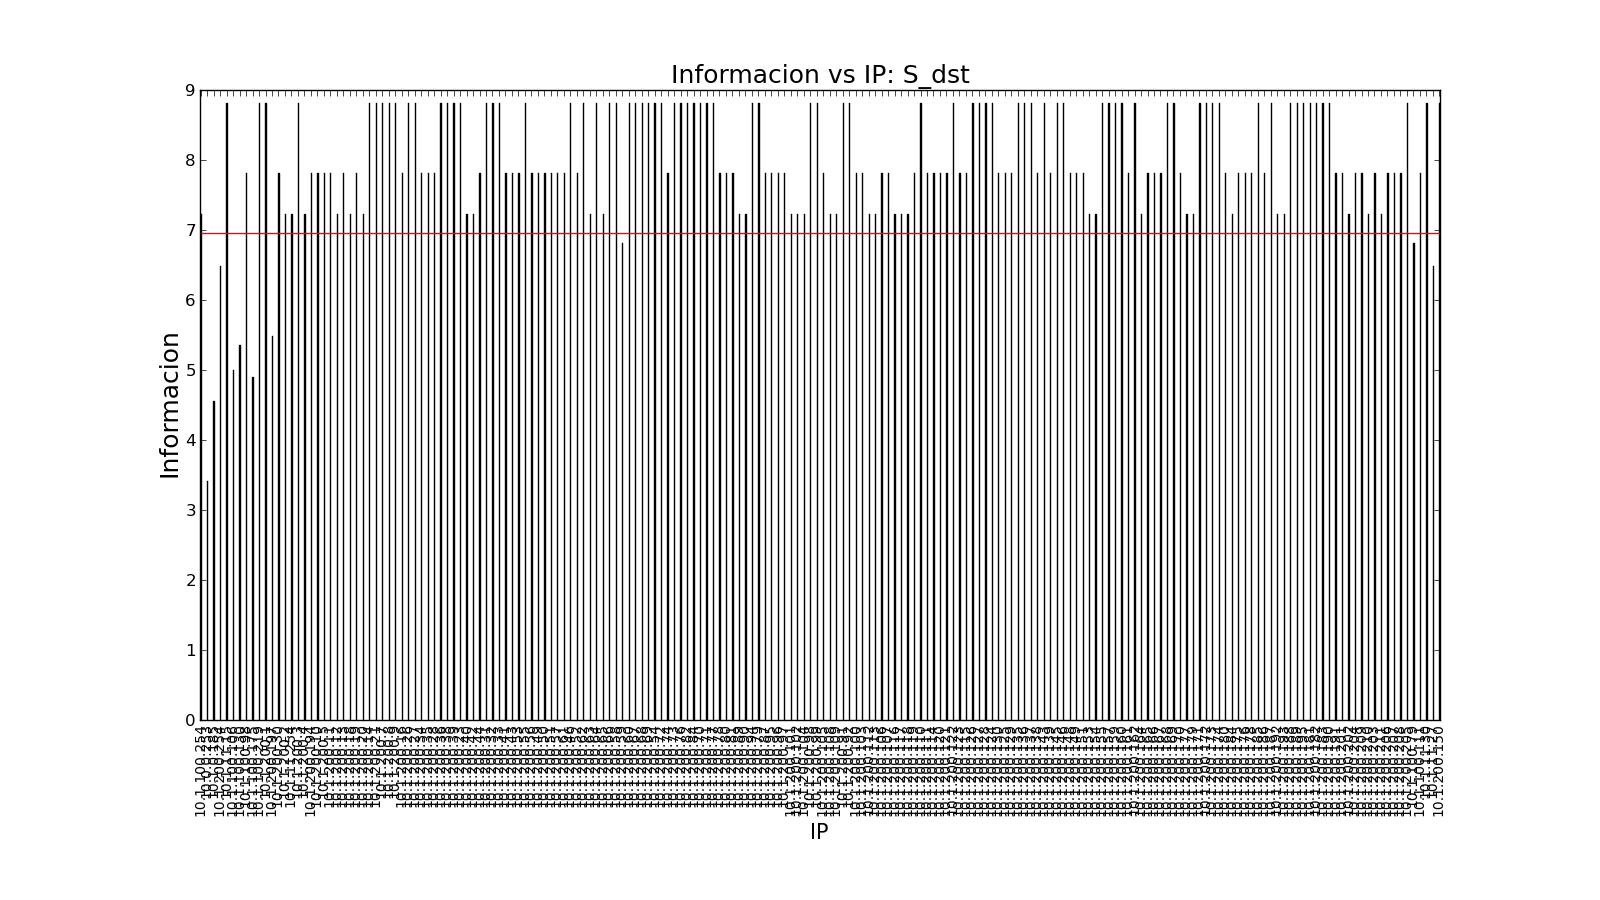
\includegraphics[width=\linewidth]{../imgs/red-entrepiso-dc_S_dst_info.png}
    \caption{Informacion de $S_{dst}$}\label{fig:entrepiso-dc-dst-info}
\end{figure}

$\bullet$ Entropía de la fuente: 6.95922916897

\subsubsection{Fuente: $S_{src}$}

\begin{figure}[H]\centering
    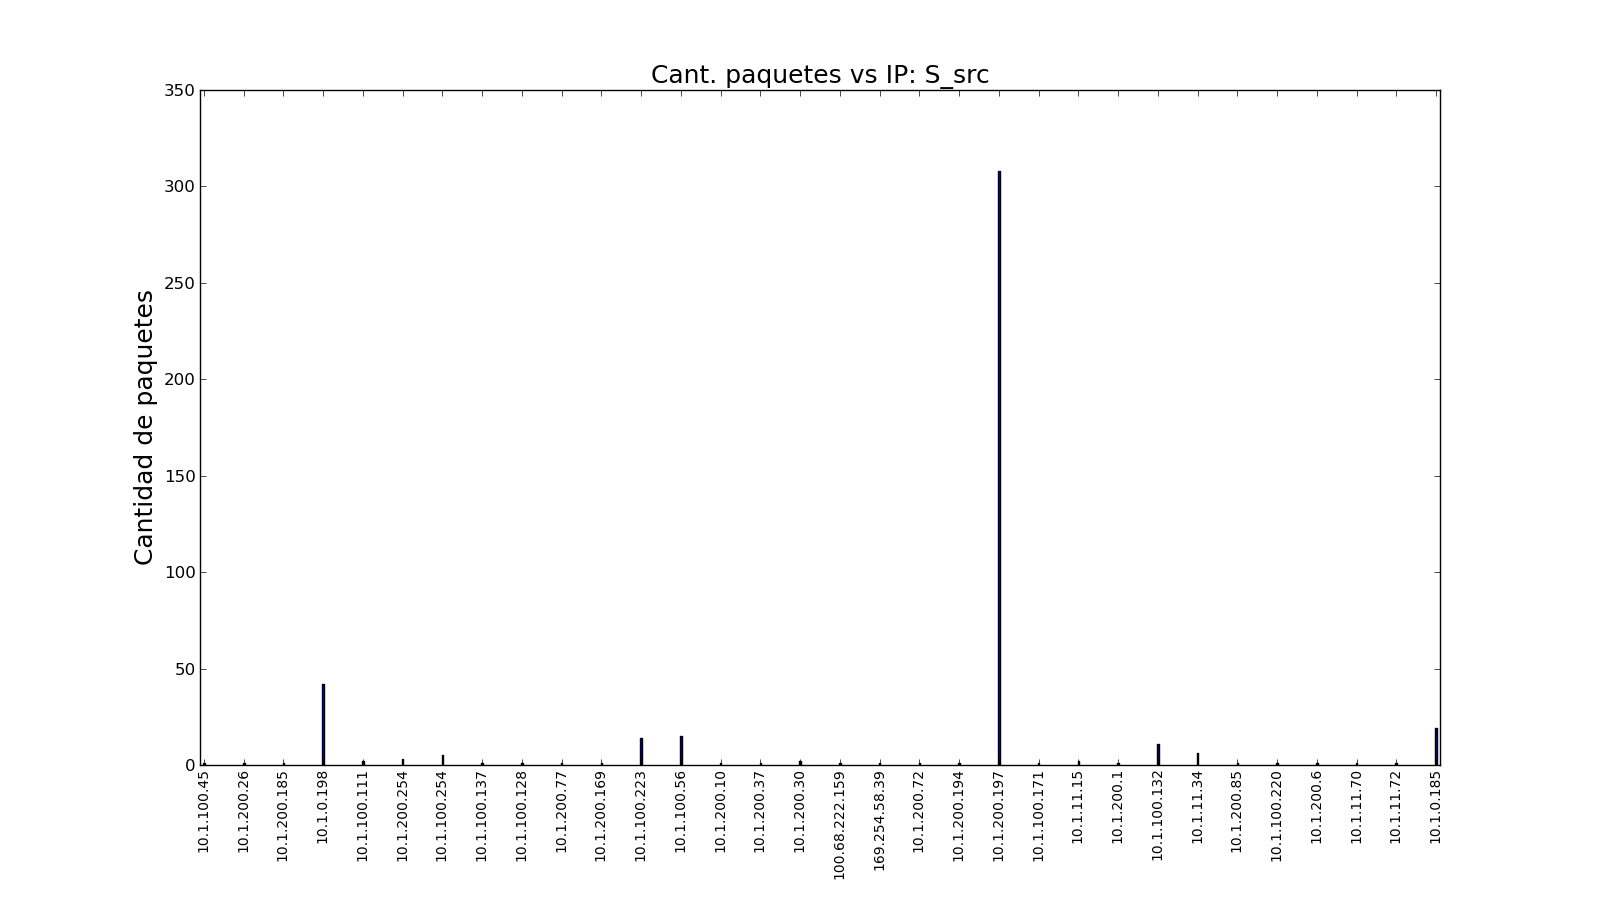
\includegraphics[width=\linewidth]{../imgs/red-entrepiso-dc_S_src_hist.png}
    \caption{Histograma de $S_{src}$}\label{fig:entrepiso-dc-src-hist}
\end{figure}

\begin{figure}[H]\centering
    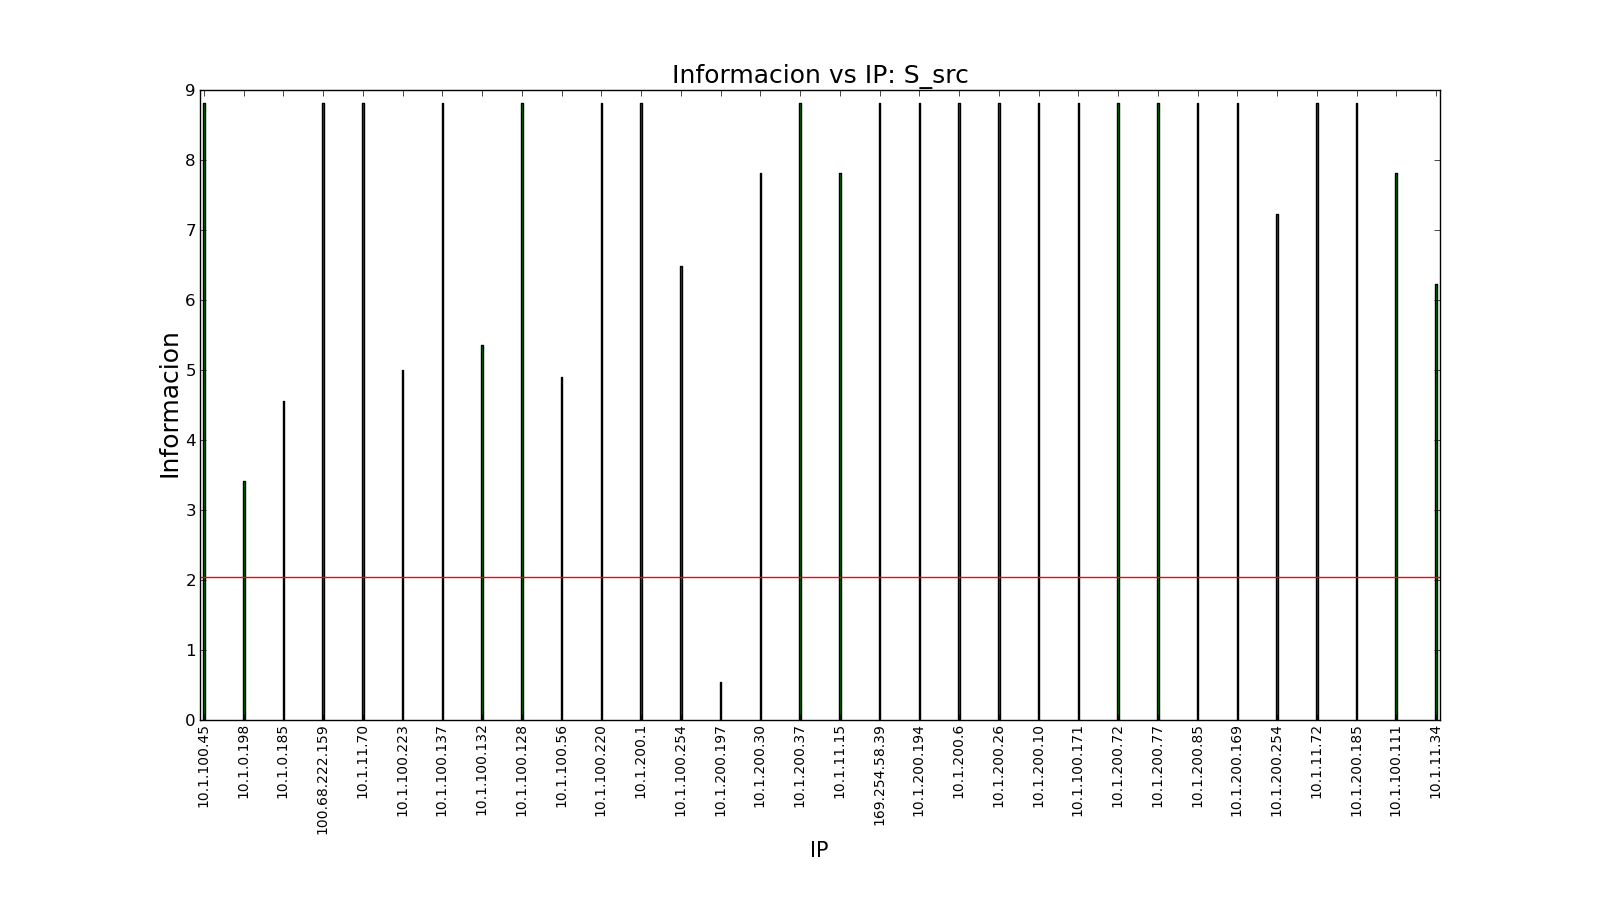
\includegraphics[width=\linewidth]{../imgs/red-entrepiso-dc_S_src_info.png}
    \caption{Informacion de $S_{src}$}\label{fig:entrepiso-dc-src-info}
\end{figure}

$\bullet$ Entropía de la fuente: 2.03731420117

\subsubsection{Discusión}

cualquier cosa interesante sobre este caso en particular

\newpage

\section{Conclusiones}
Como conclusión, queremos recalcar que por lo general los routers son nodos distinguidos en las LANs a las que pertenecen, ya que el router funciona como \emph{gateway}. Esto se mantiene, ya sea una red pública o privada.

Como pudimos ver en los experimentos, creemos que es importante saber que un nodo distinguido no siempre es un router. En el caso de Red Entrepiso, creemos que el servidor local era un nodo distinguido.

Para finalizar, en este trabajo práctico pudimos ver que no necesariamente un nodo distinguido es distinguido tanto en $S_{src}$ como en $S_{dst}$.



\end{document}	